\section{Installation de \LaTeX}
\subsection{Installer une distribution}

\begin{tcbenumerate}[3]
    \tcbitem Aller sur la page de téléchargement de \href{https://miktex.org/download}{\bfseries\color{monrose}MikTeX - https://miktex.org/download} et choisir la version \textbf{adaptée à votre système d'exploitation}.\\
    \tcbitem \textbf{Cocher} l'option \textbf{installer les packages à la volée} ( on-the-fly ) pour permettre plus de souplesse dans les premières compilations.\\
    \tcbitem \textbf{Décocher} l'option d'installation pour tous les utilisateurs. Cela rend plus simple l'utilisation de la console MikTeX.
\end{tcbenumerate}

\subsection{Ajouter un localtexmf}

Il s'agit d'un \acc{répertoire} respectant une \acc{structure précise} qui, une fois configuré est automatiquement utilisable par le compilateur \LaTeX\ comme \acc{dossier de packages}.
\begin{MultiColonnes}{2}
    \tcbitem Suivre les étapes suivantes \textbf{une seule fois} :
    \begin{tcbenumerate}
        \tcbitem Coller le dossier \textbf{localtexmf} récupéré sur ma \vocnoindexref{https://github.com/Romain1099/BFCours/tree/7f394e248e9647fe99ff78c01aaf89658ccf6b6d}{page GitHub} \textbf{n'importe ou sur votre machine}. L'essentiel est qu'il reste à cet emplacement. 
        \tcbitem Copier le chemin d'accès de ce dossier. \\
        \tcbitem Ouvrir la \bouton{console MikTeX} et aller au menu \bouton{Settings}.
        \tcbitem Aller dans l'onglet \frquote{Directories}.
        \tcbitem Appuyer sur le bouton \bouton{+} et \textbf{coller} le chemin d'accès au dossier \textbf{localtexmf}.
        \tcbitem Confirmer les changements et quitter la console. 
    \end{tcbenumerate}
    \tcbitem[valign=center] \dirtree{%
        .1 localtexmf/.
        .2 tex/.
        .3 latex/.
        .4 MonPackage/.
        .5 \textcolor{red}{MonPackage.sty}\DTcomment{fichier principal}.
        .5 fichier\_de\_package.sty.
    }
    \begin{center}
        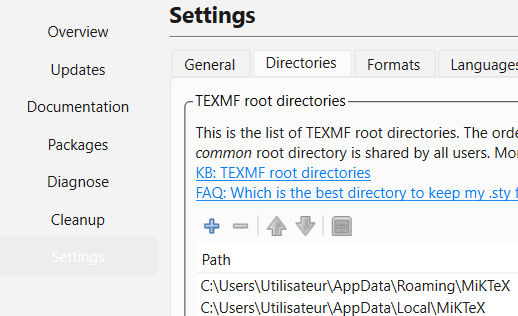
\includegraphics[width=0.75\textwidth]{images/miktex/set_localtexmf_path.png}
    \end{center}
\end{MultiColonnes}

\subsection{Installer VSCode}

Le logiciel VSCode peut être remplacé par un autre IDE s'appuyant sur cette technologie comme \acc{windsurf} ou \acc{cursor}.


\begin{tcbenumerate}[3]
    \tcbitem Aller sur la page de téléchargement de \href{https://code.visualstudio.com/download}{\bfseries\color{monrose}VSCode - https://code.visualstudio.com/download} et choisir la version \textbf{adaptée à votre système d'exploitation}.\\
    \tcbitem Laisser dans un premier temps les paramètres par défaut.
    \tcbitem Il est possible de consulter des \acc{tutoriels} en vidéo pour éditer le \acc{style} de l'IDE. 

    Tout est personnalisable.
\end{tcbenumerate}



\subsection{Installer les extensions VSCode}



\begin{MultiColonnes}{2}
    \tcbitem Puisque VSCode est un outil à \acc{destination des développeurs}, il dispose de nombreuses extensions. 

Il convient d'explorer la bibliothèque d'extension qui prend la forme d'une \acc{marketplace}. 

Par \acc{précaution}, on se limitera à des extensions téléchargées de nombreuses fois et ayant \acc{plusieurs étoiles}. 

    \tcbitem[halign=center] 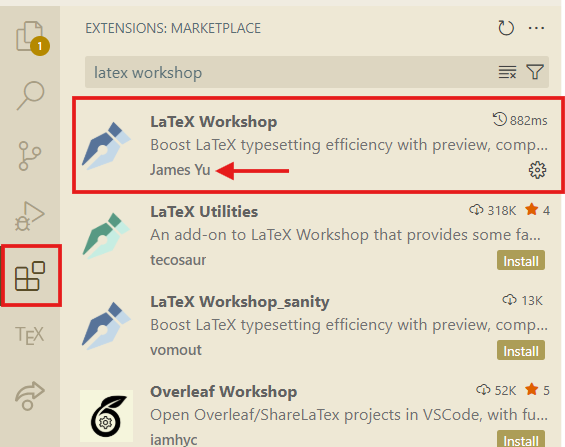
\includegraphics[width=0.75\textwidth]{images/IDE/extension_marketplace.png}
\end{MultiColonnes}


Il y a assez peu d'extensions à télécharger : 

\begin{None}
    \begin{tcbenumerate}[2]
        \tcbitem \acc{LaTeX Workshop}

        Inclut toutes les fonctionnalités de compilation automatique, visualisation de pdf.
        \begin{center}
            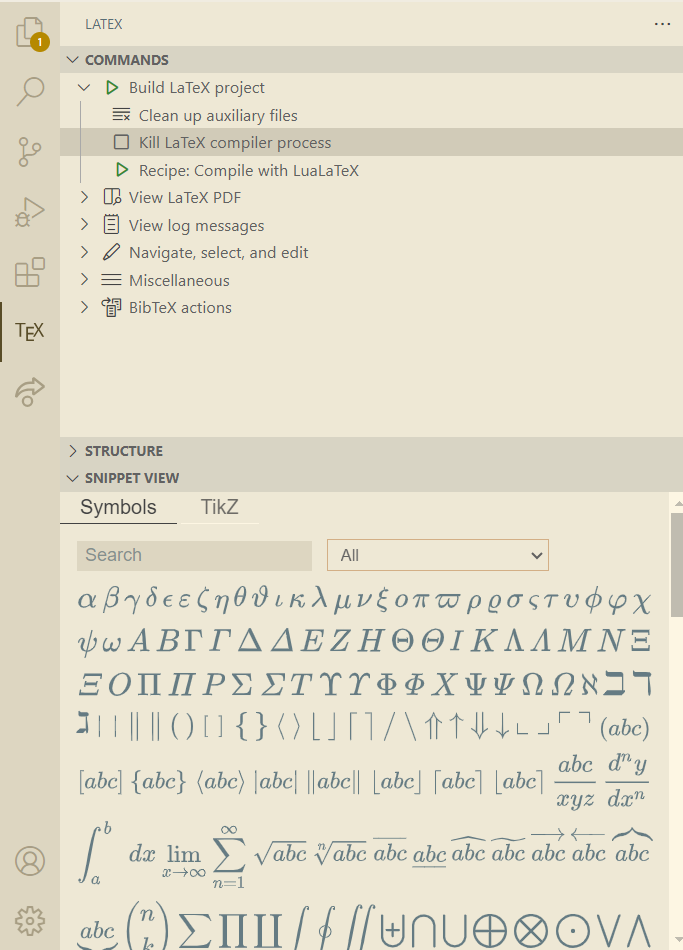
\includegraphics[width=0.9\textwidth]{images/IDE/latex_workshop.png}
        \end{center}

        \tcbitem \acc{git} 

        Pour le suivi et la gestion des modifications. C'est un incontournable surtout lorsqu'on utilise activement des agents IA. 

        \begin{center}
            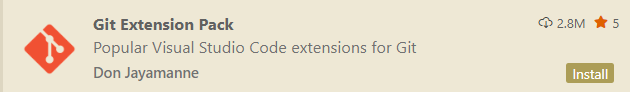
\includegraphics[width=8cm]{images/IDE/git_extension_pack.png}
        \end{center}

        \begin{Remarque}[Compilation dans VSCode]

            Il est nécessaire d'\acc{expliquer} à VSCode vos préférences de compilation. 

            Pour cela : 

            \begin{tcbenumerate}[1][1][alph]
                \tcbitem Ouvrir les \acc{settings} de l'extension \acc{LaTeX Workshop}. 

                \bouton{Barre de recherche} $\Longrightarrow$ \bouton{>latex workshop settings} $\Longrightarrow$ \bouton{>settings Sync: Open User Settings(JSON)} 

                \tcbitem Ouvrir le fichier json de settings et \acc{coller} le contenu du fichier ci-après. 

                \tcbitem Désormais, à chaque sauvegarde, le fichier se compile automatiquement et son affichage dans le prévisualisateur pdf est automatiquement actualisé. 
            \end{tcbenumerate}

        \end{Remarque}
        \tcbitem[raster multicolumn=2]  Sur VSCode, il est possible de \acc{partager une session de travail} entre 
        
        \begin{MultiColonnes}{3}
                \tcbitem[raster multicolumn=2] plusieurs participants via l'extension \voc{Live Share}.
                
                Il suffit de lire le \frquote{README} du projet pour se rendre compte de la facilité d'utilisation.
                \tcbitem[halign=center] 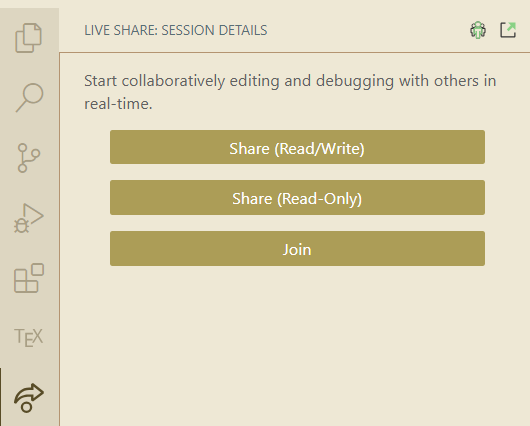
\includegraphics[width=0.55\textwidth]{images/IDE/live_share_snippet.png}
            \end{MultiColonnes}
    \end{tcbenumerate}
\end{None}

\newpage

\begin{Exemple}[Organiser vscode]

    Une fois configuré, votre environnement de travail devrait ressembler à ceci : 

    \begin{center}
        \begin{tikzpicture}
            % Image de base
            \node[anchor=center, inner sep=0] (image) at (0,0) {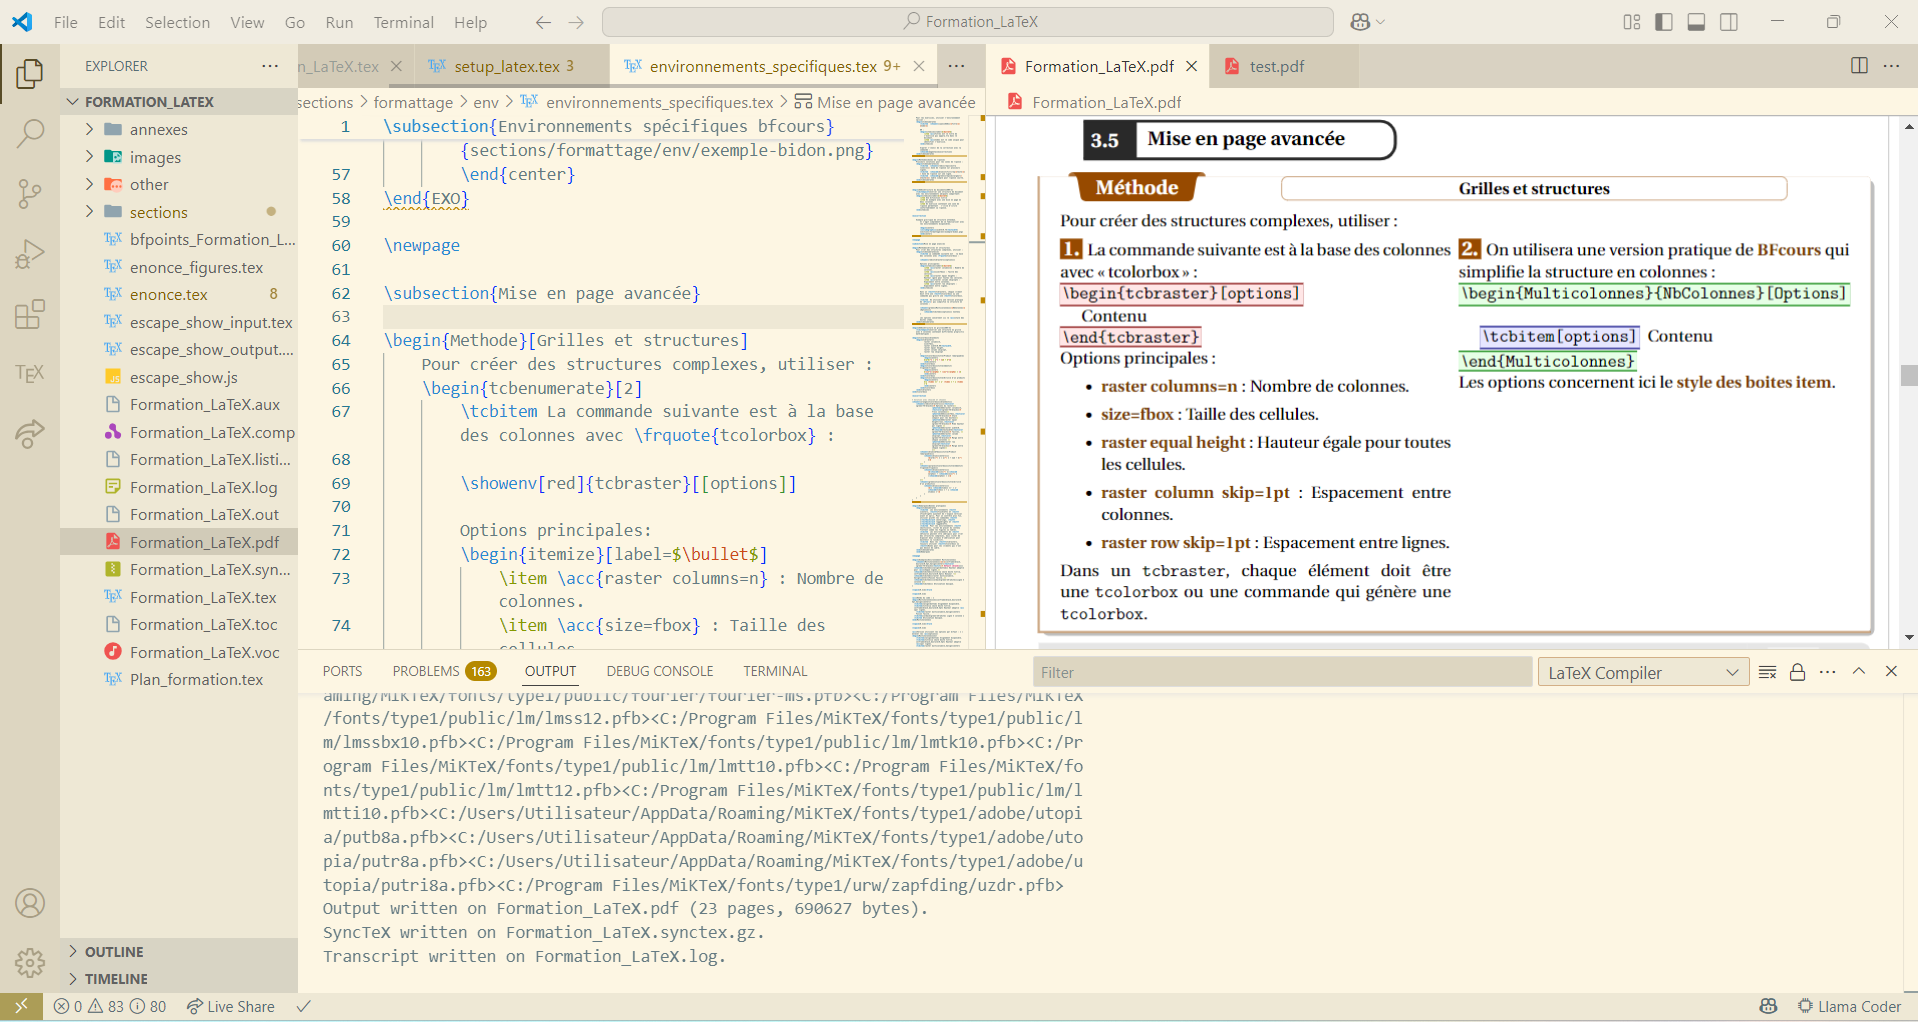
\includegraphics[width=0.8\textwidth]{images/IDE/VSCode_use.png}};
            
            % Obtenir les dimensions de l'image
            \pgfgetlastxy{\maxx}{\maxy}
            
            % Style pour les pastilles
            \tikzset{
                pastille/.style={
                    circle, 
                    fill=red!90!black, 
                    text=white, 
                    font=\bfseries\footnotesize,
                    minimum size=20pt,
                    inner sep=0pt,
                    draw=white,
                    line width=1.5pt
                }
            }
            
            % Placement des pastilles (positions relatives à l'image)
            % 1. Options générales - coin supérieur gauche
            \node[pastille] at (-7, 3.7) {1 $\rightarrow$};
            
            % 2. Barre de recherche - centre haut
            \node[pastille] at (0, 3.8) {2};
            
            % 3. Géométrie voulue pour le terminal - bas
            \node[pastille] at (4.2, 3.7) {3};
            
            % 4. La sidebar - gauche
            \node[pastille] at (-7, 0.5) {4 $ \uparrow $};
            
            % 5. Zone d'exploration - gauche dans la sidebar
            \node[pastille] at (-6, 1.5) {5};
            
            % 6. Onglets - haut du contenu principal
            \node[pastille] at (-2, 3) {6};
            
            % 7. Zone de saisie principale - centre
            \node[pastille] at (-2.5, 0) {7};
            
            % 8. Zone d'affichage secondaire - droite
            \node[pastille] at (3.5, 0) {8};
            
            % 9. Terminal - tout en bas
            \node[pastille] at (0, -2.2) {9};
        \end{tikzpicture}
    \end{center}

    On observe : 
    \begin{tcbenumerate}[2]
        \tcbitem Options générales
        \tcbitem Barre de recherche
        \tcbitem Géométrie voulue pour le terminal
        \tcbitem La \acc{sidebar}
        \tcbitem La zone d'exploration ( fichiers, extensions, recherche sur fichiers multiples )
        \tcbitem Onglets
        \tcbitem Zone de saisie principale
        \tcbitem Zone d'affichage ou de saisie secondaire
        \tcbitem Terminal - permet également d'afficher les logs : 

        \bouton{OUTPUT}$\rightarrow$\bouton{Latex Compiler}
    \end{tcbenumerate}
\end{Exemple}

\newpage

\begin{lstlisting}[language=json]
{
    "terminal.explorerKind": "external",
    "terminal.external.windowsExec": "\"C:\\Windows\\System32\\WindowsPowerShell\\v1.0\\powershell.exe\"",
    "terminal.integrated.shellIntegration.enabled": false,
    "terminal.integrated.env.windows": {
        "PATH": "${env:PATH};C:\\Program Files (x86)\\sox-14-4-2"
    },
    "latex-workshop.latex.tools": [
    {
      "name": "lualatex",
      "command": "lualatex",
      "args": [
        "-synctex=1",
        "-interaction=nonstopmode",
        "-file-line-error",
        "%DOC%"
      ]
    }
  ],
  "latex-workshop.latex.recipes": [
    {
      "name": "Compile with LuaLaTeX",
      "tools": ["lualatex"]
    }
  ],
  "latex-workshop.latex.autoBuild.run": "onSave",
  "editor.wordWrap": "on",
  "editor.cursorBlinking": "expand",
  "editor.cursorSmoothCaretAnimation": "on",
  "workbench.iconTheme": "material-icon-theme",
  "editor.mouseWheelZoom": true,
  "github.copilot.enable": {
    "*": false,
    "plaintext": false,
    "markdown": false,
    "scminput": false,
    "latex": false
  },
}
\end{lstlisting}

\newpage

\begin{EXO}{Le fameux 'Hello world !'}{SET-1}

    \begin{tcbenumerate}
        \tcbitem Ouvrir le fichier \displayFilePath{fichiers\_de\_la\_formation/1.Exercices\_formattage/hello\_world/hello\_world.tex}.
        \tcbitem Appuyer sur \bouton{CTRL+s} ou \bouton{Compiler} pour compiler ce document. 
    \end{tcbenumerate}

    \begin{bfbox}{Structure d'un document latex}
        \showcmd{documentclass}[[a4paper,11pt,fleqn]\{article\}]\mycomment{Définition de la classe du document}\\

        \mycomment{Définition de la géométrie du document}\\
        \showcmd{usepackage}[[left=1cm,right=1cm,top=0.5cm,bottom=2cm]\{geometry\}]\\

        \mycomment{Appel des packages}\\
        \showcmd{usepackage}[[french]\{babel\}] \mycomment{Options spécifiques à la langue française}\\
        \showcmd{usepackage}[\{xcolor\}] \mycomment{Utilisation des couleurs}\\
        \showcmd{usepackage}[\{fourier\}] \mycomment{Police de caractère}\\

        \mycomment{Définition de commandes}\\
        \showcmd[purple]{newcommand}[\{$\backslash$tester\}\{test\}]\\

        \mycomment{Début du document}\\
        \showcmd[red]{begin}[\{document\}] \\

        \phantom{AAA}Hello world !\\

        \phantom{AAA}\showcmd[purple]{tester} \mycomment{\'Ecrira 'test'}\\

        \showcmd[red]{end}[\{document\}]\mycomment{Fin du document}
    \end{bfbox}
\end{EXO}

\newpage
\section{Outils de formattage du texte}
\subsection{Commandes usuelles}

\begin{Methode}[Formattage du texte]
    Les commandes suivantes permettent d'effectuer la plupart des opérations sur le texte. 
    \begin{tcbenumerate}[2]
        \tcbitem  \showcmd[red]{underline\{texte\}}\ Souligner.
        \tcbitem  \showcmd[green]{hl\{texte\}}\ Surligner.
        \tcbitem  \showcmd[blue]{textbf\{texte\}}\ Mettre en gras.
        \tcbitem  \{\showcmd[purple]{textcolor\{couleur\}\{texte\}}\}\ Mettre en couleur.
        \tcbitem  \showcmd[orange]{acc[couleur]\{texte\}}\ Accentuer (bf).
        \tcbitem  \showcmd[brown]{voc[couleur]\{texte\}}\ Vocabulaire (bf).
        \tcbitem  \showcmd[cyan]{textsc\{texte\}}\ Vocabulaire.
        \tcbitem  \showcmd[magenta]{fbox\{texte\}}\ Encadrer.
        \tcbitem  \showcmd[olive]{emph\{texte\}}\ Mettre en italique.
        \tcbitem  \showcmd[teal]{frquote\{texte\}}\ Citer.
        \tcbitem  \showcmd[violet]{surligner[couleur]\{texte\}}\ Surligner (bf).
        \tcbitem  \showcmd[pink]{encadrer[couleur]\{texte\}}\ Encadrer (bf).
    \end{tcbenumerate}
\end{Methode}


\begin{EXO}{Formattage du texte}{FT-1}
    \begin{tcbenumerate}
        \tcbitem Ouvrir le fichier 
        
        \displayFilePath{fichiers\_de\_la\_formation/1.Exercices\_formattage/premier\_document/premier\_document.tex}.
        \tcbitem \tcbitempoint{2}Reproduire la phrase suivante dans laquelle \acc{chaque commande} est utilisée \encadrer[green]{une seule fois} : 

        \begin{center}
            En mathématiques, on peut \underline{souligner} les éléments importants, 
            \textbf{mettre en gras} ou \acc[red]{accentuer} des mots-clés, 
            \emph{mettre en italique} les théorèmes, 
            \hl{surligner} - ou bien \surligner[purple]{surligner} - des résultats, 
            utiliser les \textsc{petites capitales} ou la {\color{green!75!black}commande} \frquote{voc} pour le\voc{vocabulaire}, 
            et \fbox{encadrer}, ou encore \encadrer[red]{encadrer} les formules essentielles.
        \end{center}

    \end{tcbenumerate}
    
\exocorrection

%le meme texte mais avec des showcmd de différentes couleurs ( correspondant aux couleurs de la méthode )
En mathématiques, on peut \showcmd[red]{underline\{souligner\}} les éléments importants, 
\showcmd[blue]{textbf\{mettre en gras\}} ou \showcmd[orange]{acc[red]\{accentuer\}} des mots-clés, 
\showcmd[olive]{emph\{mettre en italique\}} les théorèmes, 
\showcmd[green]{hl\{surligner\}} - ou bien \showcmd[violet]{surligner[purple]\{surligner\}} - des résultats, 
utiliser les \showcmd[cyan]{textsc\{petites capitales\}} ou la \{\showcmd[green]{color\{green!75!black\}commande}\} \showcmd[teal]{frquote\{voc\}} pour le\showcmd[brown]{voc\{vocabulaire\}}, 
et \showcmd[magenta]{fbox\{encadrer\}}, ou encore \showcmd[pink]{encadrer[red]\{encadrer\}} les formules essentielles.

\begin{Remarque}
\begin{tcbenumerate}
    \tcbitem  Les commandes \frquote{acc}, \frquote{encadrer}, \frquote{surligner} sont relatives au package \bfcours.
    \tcbitem  La commande color doit être entourée par des crochets. Dans le cas contraire, la commande agit sur tout le paragraphe. 
\end{tcbenumerate}
\end{Remarque}
\end{EXO}



\subsection{Commandes personnelles}

\begin{Methode}[Définir une commande]
    Pour définir une macro on peut utiliser la syntaxe ci-dessous.
    \begin{tcbenumerate}[2]
        \tcbitem  \showcmd[purple]{newcommand\{<N>\}[<Nb>][<V>]\{<C>\}}

        Où : 
        \begin{itemize}[label=$\bullet$]
            \item \acc{<N>} est le \acc{nom} de la commande précédé d'un \frquote{backslash}.
            \item \acc{<Nb>} est le nombre de paramètres
            \item \acc{<V>} est la \acc{valeur par défaut} du premier paramètre.
            \item \acc{<C>} est le contenu de la commande.
        \end{itemize}
        Dans ce cas le premier paramètre peut être optionnel et assigné à une valeur par défaut. 

        Utiliser pour les commandes simples.

        \tcbitem  \showcmd[purple]{NewDocumentCommand\{<N>\}\{<P>\}\{<C>\}}

        Où : 
        \begin{itemize}[label=$\bullet$]
            \item \acc{<N>} est le \acc{nom} de la commande précédé d'un \frquote{backslash}.
            \item \acc{<P>} sont les paramètres définis par O\{valeurParDéfaut\} pour les paramètres optionnels, et \acc{m} pour les paramètres obligatoires.
            \item \acc{<C>} est le contenu de la commande.
        \end{itemize}
        Utiliser pour les commandes complexes.
    \end{tcbenumerate}
\end{Methode}
\newpage

\begin{EXO}{Définir une commande}{FT-2}
    \begin{tcbenumerate}[2]
        \tcbitem \tcbitempoint{1} \acc{Définir} une commande sans paramètre permettant de : 
        \begin{itemize}[label=$\bullet$]
            \item Afficher le texte \frquote{Unité non présente}.
            \item Le texte doit être en \acc{gras}. 
            \item Le texte doit être coloré en \acc{rouge}.
        \end{itemize}
        \tcbitem \tcbitempoint{1} \acc{Définir} une commande a un paramètre permettant de 
        \begin{itemize}[label=$\bullet$]
            \item Afficher le texte \frquote{Bonjour <p>} dans lequel <p> est le paramètre de la commande.
            \item Le texte doit être en \acc{gras}. 
            \item Le texte doit être coloré en \acc{vert}.
        \end{itemize}
    \end{tcbenumerate}

    \exocorrection

    \begin{tcbenumerate}
        \tcbitem Pour définir une commande sans paramètre qui affiche le texte \frquote{Unité non présente} en gras et en rouge :
        
        \showcmd[orange]{newcommand}\{\showcmd[orange]{uniteAbsente}\}\{\}
        
        \showcmd[red]{textcolor\{red\}\{\}}
        
        \showcmd[blue]{textbf\{Unité non présente\}}
        
        \showcmd[orange]{newcommand}\{\showcmd[orange]{uniteAbsente}\}\{\showcmd[orange]{textcolor\{red\}}\{\showcmd{textbf\{Unité non présente\}}\}\}
        
        \tcbitem Pour définir une commande à un paramètre qui affiche \frquote{Bonjour <p>} en gras et en vert :
        
        \showcmd[blue]{newcommand}\{\showcmd{bonjour}\}[1]\{\}
        
        \showcmd[green]{textcolor\{green\}\{\}}
        
        \showcmd[teal]{textbf\{Bonjour \#1\}}
        
        \showcmd[purple]{newcommand}\{\showcmd{bonjour}\}[1]\{\showcmd[purple]{textcolor\{green\}}\{\showcmd[purple]{textbf\{Bonjour \#1\}}\}\}
    \end{tcbenumerate}
\end{EXO}

% !TEX root = ../main.tex
\subsection{Environnements usuels}

\begin{Methode}[Formattage avec environnements]
    Les environnements suivants permettent d'effectuer la plupart des opérations de mise en page.
    \begin{tcbenumerate}[2]
        \tcbitem  \showenv[red]{center}\ Centrer un texte/contenu.
        \tcbitem  \showenv[green]{flushleft}\ Aligner à gauche.
        \tcbitem  \showenv[blue]{flushright}\ Aligner à droite.
        \tcbitem  \showenv[purple]{multicols}[\{n\}][
            Contenu gauche\\
            \showcmd{columnbreak}\\
            Contenu droit
        ]\ Affichage sur $n$ colonnes avec les packages standard.
        \tcbitem  \showenv[brown]{tcolorbox}[[options]]\ une boite.
        \tcbitem  \showenv[orange]{minipage}[\{0.475$\backslash$textwidth\}]\ une petite page dans la page.
        \tcbitem  \showenv[cyan]{itemize}[[label=\$ $\backslash$bullet\$]]\ Listes à puces.
        \tcbitem  \showenv[magenta]{enumerate}\ Listes numérotées.
        \tcbitem  \showenv[purple]{tcbenumerate}[[n][i]]\ Listes numérotées sur $n$ colonnes à partir de l'indice $i$ de bfcours.
        \tcbitem  \showenv[teal]{tabular}[[titre]\{structure\}]\ Tableaux.
        \tcbitem  \showenv[teal]{align*}\ Mode maths aligné ( séparateur \& ).
        \tcbitem  \showenv[teal]{tcbtab}[[titre]\{structure\}]\  Tableaux encadrés de bfcours.
        \tcbitem  \showenv[violet]{crep}\ Cadre de réponse (bf).
        \tcbitem  \showenv[pink]{MultiColonnes}[\{n\}[options]]\ Disposition en $n$ colonnes avec boites de style \frquote{options} (bf).
    \end{tcbenumerate}
\end{Methode}

\newpage

\begin{EXO}{Mise en page avec environnements}{ENV-1}
    \tcbitempoint{2}Reproduire la mise en page suivante en utilisant les environnements adéquats :

\begin{center}
\fbox{\begin{minipage}{0.9\textwidth}
\begin{center}
\textbf{Les différents types d'alignements}
\end{center}

\vspace{-0.25cm}\begin{multicols}{2}
\begin{flushleft}
Ce texte est aligné à gauche grâce à l'environnement \texttt{flushleft}.
\end{flushleft}

\columnbreak

\begin{flushright}
Ce texte est aligné à droite grâce à l'environnement \texttt{flushright}.
\end{flushright}
\end{multicols}

\vspace{-1cm}\begin{center}
Ce texte est centré grâce à l'environnement \texttt{center}.
\end{center}

\begin{tcbtab}[Résumé des environnements d'alignement]{|l|c|r|}
\hline
\textbf{Environnement} & \textbf{Description} & \textbf{Utilisation} \\
\hline
flushleft & Aligne à gauche & Texte courant \\
center & Centre le texte & Titres, équations \\
flushright & Aligne à droite & Signature, date \\
\hline
\end{tcbtab}
\end{minipage}}
\end{center}

\exocorrection

\showenv{center}[][
	 \showenv{minipage}[\{0.9$\backslash$textwidth\}][
		 \showenv{center}[][
		 	\showcmd{textbf}[Les différents types d'alignements]
		]\\
		\showenv{multicols}[\{2\}][
			\showenv{flushleft}[][
				Ce texte est aligné à gauche grâce à l'environnement \encadrer{flushleft}.
			]\\
			\showcmd{columnbreak}[]\\
			\showenv{flushright}[][
		 		Ce texte est aligné à droite grâce à l'environnement \encadrer{flushright}.
			]
		]\\
        \showenv{center}[][
            \showenv{tcbtab}[[Résumé des environnements d'alignement]\{|l|c|r|\}][
                \showcmd{hline}\\
                flushleft \& Aligne à gauche \& Texte courant $\backslash$$\backslash$\\
                center \& Centre le texte \& Titres, équations $\backslash$$\backslash$\\
                flushright \& Aligne à droite \& Signature, date $\backslash$$\backslash$\\
                \showcmd{hline}
            ]
        ]
	]
]
\end{EXO}



\subsection{La géométrie}
\begin{Methode}[Géométrie et \LaTeX]
        
        L'utilisation de la géométrie repose essentiellement sur le package \acc{TikZ}. 

        Son utilisation est \acc{omniprésente} en \LaTeX\ - la bordure de cet environnement est \acc{dessinée} avec une figure TikZ.

        Malheureusement, la maîtrise de ce package nécessiterait une formation à part entière (- cf. sa documentation CTAN et les ouvrages associés \acc{TikZ pour l'impatient} ou bien le package \acc{tkz-euclid}.\\


        Néanmoins, le professeur de mathématiques sera ravi d'apprendre que le logiciel de géométrie dynamique \acc{Geogebra} ou d'autres comme celui du groupe \acc{coopmaths} permettent un \acc{export TikZ} des figures réalisées. 

        \vspace{-0.45cm}\begin{center}
            \bouton{Fichier}$\longrightarrow$\bouton{Exporter}$\longrightarrow$\bouton{Graphique vers PGF/TikZ}
        \end{center}

        \vspace{-0.3cm}Il suffit ensuite de se laisser guider par l'interface proposée par Geogebra.

        On veillera à copier coller le contenu généré \acc{entre les bornes} \showcmd{begin\{document\}} et \showcmd{end\{document\}}.

        L'utilisation d'un \acc{script de reformattage} des figures TikZ ainsi générée est \acc{hautement conseillé} - les outils de \bfcours\ proposent un tel programme adapté à plusieurs situations. 
    \end{Methode}
\subsection{Le mode mathématiques}

\begin{Methode}[Mode mathématique]
    Le \voc{mode mathématique} permet l'accès aux commandes de calcul et \acc{adapte} la police aux mathématiques. 

    Pour une \acc{documentation}, on peut conseiller : \vocnoindexref{https://math.univ-lyon1.fr/irem/spip.php?article340}{LaTeX pour le prof de maths} ou encore \vocnoindexref{https://tug.ctan.org/info/short-math-guide/short-math-guide.pdf}{Petit guide des mathématiques - CTAN}. 


    On l'utilise de plusieurs manières ayant chacune leur spécificité. 

    \begin{MultiColonnes}{2}[colframe=\itemBaseColor,boxrule=0.4pt]
        \tcbitem[title=Mode basique] S'utilise via : \$ $contenu\  maths$ \$

        $\rightarrow$ S'insère dans le texte.

        $\rightarrow$ Simple à utiliser. 
        \tcbitem[title=Mode étendu] S'utilise via : $\backslash$( $contenu\  maths$ $\backslash$)

        $\rightarrow$ S'insère dans le texte.

        $\rightarrow$ Tailles plus importantes ( fractions ). 
        \tcbitem[title=Mode display centré] S'utilise via : $\backslash$[ $contenu\  maths$ $\backslash$]

        $\rightarrow$ Saute une ligne et indente.

        $\rightarrow$ Tailles plus importantes ( fractions ). 
        \tcbitem[title=Mode equation / align]  \showenv[red]{align*}[][$contenu\ \& \  maths$]
    \end{MultiColonnes}
\end{Methode}
\newpage
\section{Utiliser un package didactique}
\subsection{Introduction}


L'on dit toujours que le plus important lorsque l'on programme un logiciel ou un document, ce sont les \acc{contenants}. 

En effet, de bons contenants automatisent certaines fonctionnalités que l'auteur souhaite retrouver en tous temps. 
C'est précisément ce qui bloque de nombreux adeptes de \LaTeX. 

De nombreux packages sont disponibles et proposent des fonctionnalités plus ou moins équivalentes à celles développées dans \bfcours. 

Dans la suite de cette formation, nous utiliserons \bfcours\ par soucis d'homogénéité de la formation, mais il est tout à fait possible d'utiliser un autre package didactique à la place. 

Cela permet d'introduire la sous-section la plus importante de cette formation : \acc{la documentation}.

\subsection{Se documenter}

\begin{EXO}{Utiliser la documentation}{BF-3}
    Explorez l'univers de la communauté \LaTeX\ en découvrant deux packages didactiques comme alternatives à \bfcours. 

    \begin{tcbenumerate}[2]
        \tcbitem \tcbitempoint{1} Utiliser le package \encadrer[red]{pas-cours}.
        \begin{itemize}[label=$\bullet$]
            \item \acc{Accéder} à la documentation de \acc{pas-cours} sur \vocnoindexref{https://ctan.org/pkg/pas-cours}{CTAN - \frquote{pas-cours}}.
            \item \acc{Repérer les environnements didactiques}. 
            %\item Les \acc{utiliser} dans un exemple basique. 
        \end{itemize}
        \tcbitem \tcbitempoint{1} \acc{Utiliser} le package \encadrer[red]{profMaquette}. 
        \begin{itemize}[label=$\bullet$]
            \item Aller sur le site \vocnoindexref{https://ctan.org/}{https://ctan.org/}
            \item Chercher la documentation du package \frquote{profMaquette} de \acc{Christophe Poulain}. 
            %\item Construire un nouveau document latex utilisant ce package. 
        \end{itemize}
    \end{tcbenumerate}
    \exocorrection

    Cette correction n'est pas implémentée. 

    Il s'agit d'une alternative à l'utilisation de \bfcours.
\end{EXO}
\input{sections/activite_chose_didactic_package.tex}
\subsection{Compiler un document avec bfcours}

\begin{Methode}[Première compilation avec bfcours]

    L'architecture recommandée pour éditer des documents \LaTeX\ est la suivante : 
    \begin{tcbraster}[raster columns=3,blank]
        \begin{tcolorbox}[blank,raster multicolumn=2]
            \dirtree{%
                .1 \textbf{NomPrincipal}.
                .2 \textcolor{blue}{images/}\DTcomment{Dossier pour toutes les images}.
                .2 \textcolor{blue}{sections/}\DTcomment{Optionnel pour les gros fichiers}.
                .2 \textcolor{blue}{annexes/}\DTcomment{Optionnel, documents auxiliaires}.
                .3 scripts/.
                .3 csv/.
                .3 todolists/.
                .2 \textbf{NomPrincipal.tex}\DTcomment{Fichier principal à compiler}.
                .2 enonce.tex\DTcomment{Contenu principal, organise les sous-fichiers}.
                .2 enonce\_figures.tex\DTcomment{Contient les figures TikZ du projet}.
            }

            Les répertoires en \encadrer{bleu} sont présents en cas de nécessité seulement.
        \end{tcolorbox}
        \begin{tcolorbox}[blank] 
            Cette organisation permet de :
            \begin{itemize}[label=$\bullet$]
                \item Séparer clairement le contenu de la structure : les en-têtes sont dans le \acc{fichier principal} et le contenu est dans \acc{enonce.tex}.
                \item Produire différentes versions pour un même contenu ( A3, dys, corrections, élève... )
                \item Faciliter la maintenance et les modifications
                \item Réutiliser des éléments entre différents projets
            \end{itemize}
        \end{tcolorbox}
    \end{tcbraster}


    Pour \voc{compiler} un document \LaTeX\ avec bfcours, il suffit de : 
    \begin{tcbenumerate}
        \tcbitem \tcbitempoint{1} \'Ecrire le contenu dans un fichier nommé \acc{enonce.tex}
        \tcbitem \tcbitempoint{1} Compiler le \acc{fichier principal} en utilisant \acc{LuaLaTeX} - sinon ça ne compile pas. 
    \end{tcbenumerate}
\begin{Remarque}
    LuaLaTeX est un compilateur permettant de compiler avec le moteur \LaTeX\ tout en autorisant l'utilisation de scripts écrits en langage Lua. 

    Ce langage est simple et fonctionne sur tous les hardware, mais n'est pas autorisé par défaut dans les compilateurs \LaTeX.
\end{Remarque}
\end{Methode}

\begin{EXO}{Première compilation avec bfcours}{BF-1}

    \itempoint{1}Accéder au répertoire \displayFilePath{fichiers\_de\_la\_formation/2.Exercices\_bfcours}.

    \itempoint{1}Ouvrir son fichier principal \displayFilePath{fichiers\_de\_la\_formation/1.Exercices\_bfcours/Exercices\_bfcours.tex} avec \acc{VScode} ( ou l'\voc{IDE} de votre choix ).

    \itempoint{1}Compiler le fichier.
    
    \exocorrection

    Il faut compiler avec \acc{LuaLaTeX}.
\end{EXO}
\subsection{Utiliser les environnements didactiques}

\begin{MultiColonnes}{2}
    \tcbitem Le package \bfcours\ propose des \acc{environnements didactiques} destinés à la transmission de connaissances. 

    Ils s'utilisent de manière très simple mais agissent à plusieurs niveau et sont l'aboutissement de beaucoup de travail.
    \tcbitem \begin{itemize}[label=$\bullet$]
    \item Présentation claire isolant le contenu du reste du document. 
    \item Insertion dans la table des matières. 
    \item Gestion des couleurs permettant une cohérence visuelle.
    \item Gestion des marges et de la police.
    \item Pour les exercices : gestion des numéros, des corrections séparées, des points et de la difficulté.
\end{itemize}
\end{MultiColonnes}
\begin{tcolorbox}[blank]
    \begin{tcbenumerate}[2]
        \tcbitem \tcbitempoint{1} On peut donc utiliser tous les environnements suivants librement, via la syntaxe :

            \showenv[blue]{NomEnvironnement}[[titre][options]]

            \begin{itemize}[label=$\bullet$]
                \item \textbf{NomEnvironnement} : Le nom de l'environnement commence toujours par une majuscule et sans accent (Exemple : \texttt{Methode}, \texttt{Definition}, \texttt{Theoreme}).
                
                \item \textbf{Titre} : La première option correspond au titre.
                
                \item \acc{Options} : La seconde option est destinée à ajouter des options tcolorbox dans la définition de l'environnement.  
            \end{itemize}
            \begin{Remarque}
                L'environnement \acc{EXO} a une syntaxe particulière :
            
                \showenv[red]{EXO}[\{Titre\}\{Code compétence\}]
                
            \end{Remarque}
        \tcbitem[valign=top] \tcbitempoint{1}Environnements didactiques
        
        \begin{tcbtab}{p{0.24\textwidth}p{0.54\textwidth}}%

                \textcolor{meth}{\textbf{Methode}} & Pour présenter des méthodes de résolution \\
                \textcolor{defi}{\textbf{Definition}} & Pour introduire une nouvelle définition \\
                \textcolor{thm}{\textbf{Theoreme}} & Pour énoncer un théorème mathématique \\
                \textcolor{ex}{\textbf{Exemple}} & Pour illustrer par un exemple \\
                \textcolor{ex}{\textbf{EXO}} & Pour proposer un exercice \\
                \textcolor{rem}{\textbf{Remarque}} & Pour ajouter une remarque\\
                \textcolor{nota}{\textbf{Notation}} & Pour définir une notation\\
                \textcolor{demo}{\textbf{Demonstration}} & Pour ajouter une démonstration\\
                \textcolor{act}{\textbf{Activite}} & Pour ajouter une activité\\
                \textcolor{nota}{\textbf{Aide}} & Pour ajouter une aide.
            \end{tcbtab}
        %\end{tcolorbox}
    \end{tcbenumerate}
\end{tcolorbox}

\begin{EXO}{Utiliser les environnements de bfcours}{BF-3}

    \itempoint{2}\acc{\'Ecrire} un fichier contenant la \acc{Definition} d'une \acc{fraction} en utilisant bfcours.

    \begin{Aide}[Utilitaire]
            On peut utiliser les commandes suivantes : 

            \begin{tcbenumerate}[2]
                \tcbitem \showcmd[red]{dfrac\{Num\}\{Den\}} - Pour les \acc{fractions}.

                \encadrer[red]{S'utilise en \acc{mode mathématiques}}. 
                \tcbitem \showcmd[red]{red\{texte\}} - Raccourci pour écrire en rouge.
                \tcbitem \showcmd[red]{Si} - L'un des \acc{connecteurs logiques} de \bfcours.
                \tcbitem \showcmd[blue]{Alors} - L'un des \acc{connecteurs logiques} de \bfcours.
            \end{tcbenumerate}
    \end{Aide}

    \exocorrection%
    
    Code :

    \showenv[red]{Definition}[[Fraction]][%
        \showenv[cyan]{MultiColonnes}[\{3\}][%
            \showcmd[red]{tcbitem[raster multicolumn=2]} Soient deux nombres $n$ et $d$.
            Le \showcmd[red]{red\{quotient de \$n\$ par \$d\$\}}, est le \showcmd[red]{red\{résultat\}} de la \showcmd{voc\{division\}} du nombre 
            \$n\$ par le nombre \$d\$.
            Il est noté en \showcmd[green]{voc\{écriture fractionnaire\}} \$\showcmd[red]{encadrer[red]}\{\showcmd[green]{dfrac\{n\}\{d\}}\}\$.
            \showcmd[red]{Si} les nombres \$n\$ et \$d\$ sont \showcmd[purple]{acc\{entiers\}}, \showcmd[blue]{Alors} le nombre \$\showcmd[green]{dfrac\{n\}\{d\}}\$ est appelé une 
            \showcmd[green]{voc\{fraction\}}
            \showcmd[red]{tcbitem[valign=center]} \showcmd{bclampe} Le \showcmd{frquote\{trait de fraction\}} représente une \showcmd{acc\{opération de division\}}.]]

    \hrule

    \begin{Definition}[Fraction]
        \begin{tcbraster}[
            blank,
            raster columns=3, 
            raster equal height, 
            raster width=0.99\textwidth
        ]
        \begin{tcolorbox}[blank,raster multicolumn=2]
            Soient deux nombres $n$ et $d$.
        
            Le \red{quotient de $n$ par $d$}, est le \red{résultat} de la \acc{division} du nombre $n$ par le nombre $d$.
            

            Il est noté en \acc{écriture fractionnaire} \encadrer[red]{$\dfrac{n}{d}$}.

            \Si les nombres $n$ et $d$ sont \acc{entiers}, \Alors le nombre $\dfrac{n}{d}$ est appelé une \acc{fraction}.
        \end{tcolorbox}
        \begin{tcolorbox}[blank, valign=center]
            \bclampe Le \frquote{trait de fraction} représente une \acc{opération de division}.
        \end{tcolorbox}
        \end{tcbraster}
    
    \end{Definition}
\end{EXO}  
\begin{Methode}[Zones de réponse]
    Dans de trop nombreuses ressources, la gestion des \acc{espace réponse} reste trop superficielle. 
    Les environnements du package \acc{rdcrep} associés à ceux de \bfcours\ forment un ensemble permettant d'éditer des zones de réponse bienveillants.
    \begin{tcbenumerate}[2]
        \tcbitem  \showcmd[green]{repsim[largeur]\{texte\}}\ \mycomment{Cadre simple pour réponse courte.}

        
        Date : \repsim[3cm]{20/04/25} Note : \repsim[1.5cm]{10}/20
        \tcbitem  \showcmd[blue]{tcfillcrep\{texte\}}\ \mycomment{Zone de réponse extensive sur une ligne.}
        Ceci \tcfillcrep{est un} texte.

        \tcfillcrep{La même commande sur une ligne vide}
        \tcbitem  \showenv[red]{crep}[[extra lines=n]]\ \mycomment{Zone de réponse sur plusieurs lignes.}
        \begin{crep}
        Ceci est une réponse

        sur plusieurs lignes. 
        \end{crep}
        \tcbitem \showcmd[purple]{setrdcrep}%
         \{\\
            \phantom{AAAA}seyes, \mycomment{/ colback=white,}\\
            \phantom{AAAA}correction=true, \\
            \phantom{AAAA}correction color=monrose, \\
            \phantom{AAAA}correction font = $\backslash$large$\backslash$bfseries,\\
            \phantom{AAAA}tcolorbox\_options \mycomment{options supplémentaires}\\
        \} \mycomment{Style de la correction}
    \end{tcbenumerate}
\end{Methode}

\begin{EXO}{Environnements de bfcours}{BF-2}
    \tcbitempoint{2}Créer une structure de document avec les environnements adéquats comportant:
    \begin{itemize}[label=$\bullet$]
        \item Une définition titrée
        \item Un exemple avec une mise en page en deux colonnes
        \item Un exercice contenant une zone de réponse permettant à l'élève d'écrire confortablement sa réponse. 
    \end{itemize}


\exocorrection

	Exemple générique de structure attendue. 
        Il s'agit simplement de se familiariser avec les environnements disponibles. 

        \begin{center}
        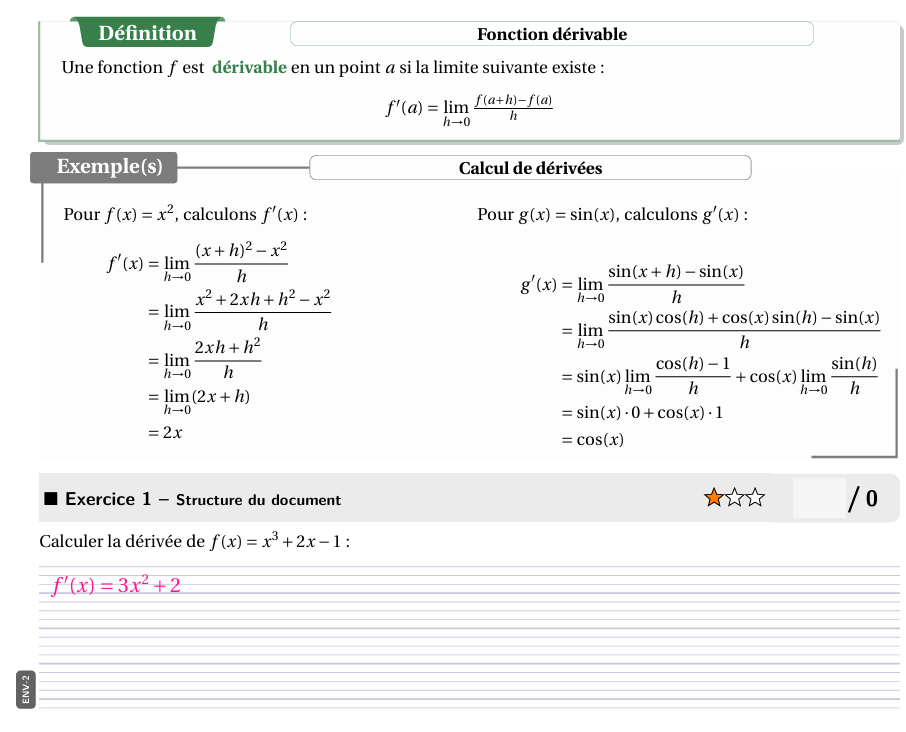
\includegraphics[width=0.75\textwidth]{sections/formattage/env/exemple-bidon.png}
        \end{center}
\end{EXO}

\newpage
\subsection{Mise en page avancée}

\begin{Methode}[Grilles et structures]
    Pour créer des structures complexes, utiliser :
    \begin{tcbenumerate}[2]
        \tcbitem La commande suivante est à la base des colonnes avec \frquote{tcolorbox} : 
        
        \showenv[red]{tcbraster}[[options]]

        Options principales:
        \begin{itemize}[label=$\bullet$]
            \item \acc{raster columns=n} : Nombre de colonnes.
            \item \acc{size=fbox} : Taille des cellules.
            \item \acc{raster equal height} : Hauteur égale pour toutes les cellules.
            \item \acc{raster column skip=1pt} : Espacement entre colonnes.
            \item \acc{raster row skip=1pt} : Espacement entre lignes.
        \end{itemize}
        
        Dans un \texttt{tcbraster}, chaque élément doit être une \texttt{tcolorbox} ou une commande qui génère une \texttt{tcolorbox}.
        
        \tcbitem  On utilisera une version pratique de \bfcours\ qui simplifie la structure en colonnes :

        \showenv[green]{Multicolonnes}[\{NbColonnes\}[Options]][
            \showcmd{tcbitem}[[options]] Contenu
        ]\\

        Commentaires : 
        \begin{itemize}[label=$\bullet$]
            \item Dispose le contenu en \acc{grille} en le stockant dans des \acc{tcolorbox}.
            \item La commande \showcmd{tcbitem} permet de changer de boite - et donc de colonne. 
            \item Les options de MultiColonnes modifient de façon globale le style des boites. 
            \item Les options de tcbitem modifie de façon locale le style de la boite. 
        \end{itemize}

    \end{tcbenumerate}
\end{Methode}

\begin{Remarque}
    Les options ci-dessus sont celles utilisables dans le package \vocref{https://ctan.org/pkg/tcolorbox}{tcolorbox}.    
    
    Puisque \acc{tout est boite}, la documentation de ce package est \acc{l'outil par exellence} pour produire du contenu de qualité et utiliser correctement les nombreuses options disponibles. 
\end{Remarque}
%\newpage
\begin{EXO}{Structure en grille}{ENV-3}
    \tcbitempoint{2}Créer une structure en grille avec 3 colonnes contenant différentes propriétés mathématiques :

\begin{tcolorbox}[blankest]
    \begin{tcbraster}[
            raster columns=3, 
            size=fbox,
            raster width=0.99\textwidth, 
            raster equal height, 
            raster column skip=1pt, 
            raster row skip=1pt
        ]
        \begin{tcolorbox}[title=Produit remarquable]
            \begin{center}
            $(a+b)^2 = a^2 + 2ab + b^2$
            \end{center}
        \end{tcolorbox}
        \begin{tcolorbox}[title=Identité trigonométrique]
            \begin{center}
            $\sin^2(\alpha) + \cos^2(\alpha) = 1$
            \end{center}
        \end{tcolorbox}
        \begin{tcolorbox}[title=Dérivée d'un produit]
            \begin{center}
            $(u \times v)' = u' \times v + u \times v'$
            \end{center}
        \end{tcolorbox}
    \end{tcbraster}
\end{tcolorbox}

\exocorrection

% Solution avec showcmd et showenv
\showenv[orange]{tcolorbox}[[blankest]][
    \showenv[red]{tcbraster}[][[\textcolor{green!75!black}{\% Options du raster}\\
                    \phantom{AAA}raster columns=3,\textcolor{green!75!black}{\% Trois colonnes}\\
                    \phantom{AAA}size=fbox,\textcolor{green!75!black}{\% Style compact pour les boites}\\
                    \phantom{AAA}raster equal height=rows,\textcolor{green!75!black}{\% Même hauteur par ligne} \\
                    \phantom{AAA}raster width=0.99\showcmd{textwidth}\textcolor{green!75!black}{\% Taille}, \\
                    \phantom{AAA}raster column skip=1pt,\textcolor{green!75!black}{\% Marge entre chaque colonne} \\
                    \phantom{AAA}raster row skip=1pt\textcolor{green!75!black}{\% Marge entre chaque ligne}\\
                    ]\\
        \showenv[blue]{bfbox}[[title=Produit remarquable]][
            \showenv[blue]{center}[][
                \$(a+b)\^\ 2 = a\^\ 2 + 2ab + b\^\ 2\$\\
            ]
        ]\\
        \showenv[purple]{tcolorbox}[[title=Identité trigonométrique]][
            \showenv[blue]{center}[][
                \$\showcmd{sin}\^\ 2(\showcmd{alpha}) + \showcmd{cos}\^\ 2(\showcmd{alpha}) = 1\$
            ]
        ]\\
        \showenv[green]{tcolorbox}[[title=dérivée d'un produit]][
            \showenv[blue]{center}[][
                \$(u \showcmd{times} v)' = u' \showcmd{times} v + u \showcmd{times} v'\$
            ]
        ]
    ]
]
\end{EXO}

\newpage

\vspace{-0.7cm}\begin{Exemple}[Environnement MultiColonnes]
    \vspace{-0.35cm}\showenv{MultiColonnes}[\{2\}[colframe=black,boxrule=0.4pt,halign=center]\textcolor{green!75!black}{\textit{\% Default [blank]}}][
  \showcmd{tcbitem}[[valign=bottom]] Hauteur adaptée pour \acc{chaque ligne}.\\
  \showcmd{tcbitem}[[title=La seule boite titrée,colframe=black,boxrule=0.4pt]] Bonjour !\\
  \showcmd{tcbitem}[[raster multicolumn=2,halign=center]]Fusion facile..\\
  \showcmd{tcbitem}[[colback=green!25!white]]Ligne 3 colonne 1\\
  \showcmd{tcbitem}[] Utilisation basique.
]

\vspace{0.2cm}\hrule

\vspace{0.2cm}

\acc{Rendu du code : }

\begin{MultiColonnes}{2}[colframe=black,boxrule=0.4pt,halign=center]%
  \tcbitem[valign=bottom] Alignement disponible.
  \tcbitem[title=La seule boite titrée,colframe=black,boxrule=0.4pt] Hauteur adaptée \acc{par ligne}.
    \tcbitem[raster multicolumn=2,halign=center] Fusion facile..
  \tcbitem[colback=green!25!white] Ligne 3 colonne 1
  \tcbitem Utilisation basique.
\end{MultiColonnes}

\vspace{0.2cm}\hrule

\vspace{0.2cm}

\acc{Version utilisant les options par défaut : } ( enlever les \acc{options})

\begin{MultiColonnes}{2}%
    \tcbitem[valign=bottom] Alignement disponible.
    \tcbitem[title=La seule boite titrée,colframe=black,boxrule=0.4pt] Hauteur adaptée \acc{par ligne}.
    \tcbitem[raster multicolumn=2,halign=center] Fusion facile..
  \tcbitem[colback=green!25!white] Ligne 3 colonne 1
  \tcbitem Utilisation basique.
\end{MultiColonnes}

\vspace{0.2cm}\hrule

\vspace{0.2cm}

\acc{Style modifié : } en utilisant un \showcmd[orange]{tcbset} précis. 

\begin{MultiColonnes}{4}%
\tcbitem[raster multicolumn=2] \showcmd[orange]{tcbset}\{\\
  \phantom{A}ColonnesBaseStyle/.style=\{\\
    \phantom{AA}top=0pt,\\
    \phantom{AA}bottom=0pt,\\
    \phantom{AA}left=0pt,\\
    \phantom{AA}right=0pt,\\
    \phantom{AA}colback=blue!5!white,\\
    \phantom{AA}colframe=blue!75!black,\\
    \phantom{AA}before title={\showcmd{dimcoloredsquare}[\{white\}\{1.5\}]},\\
    \phantom{AA}after title=\showcmd{hfill}\showcmd{today}\},\\
    \phantom{AA}boxrule=0.4pt\\
    \phantom{AA}\}\\
\}
\tcbitem[raster multicolumn=2] 
    \tcbset{
    ColonnesBaseStyle/.style={
        top=0pt,
        bottom=0pt,
        left=0pt,
        right=0pt,
        colback=blue!5!white,
        colframe=blue!75!black,
        before title={\dimcoloredsquare{white}{1.5}\ },
        after title={\ \today},
        boxrule=0.4pt
    }
    }
    \begin{MultiColonnes}{2}%
        \tcbitem[valign=bottom] Alignement disponible.
        \tcbitem[title=La seule boite titrée,colframe=black,boxrule=0.4pt] Hauteur adaptée \acc{par ligne}.
        \tcbitem[raster multicolumn=2,halign=center] Fusion facile..
        \tcbitem[colback=green!25!white] Ligne 3 colonne 1
        \tcbitem Utilisation basique.
    \end{MultiColonnes}
\end{MultiColonnes}
\end{Exemple}
\vspace{-0.7cm}


\newpage
\section{Ateliers}

\begin{Activite}[\'Elaborer un document \LaTeX\ en groupe]

    \`A travers les exercices suivants, vous apprenez à utiliser l'\acc{écosystème} \LaTeX\ ainsi que les facilités de partage de code. 

    \acc{Durée :} \hspace{1cm}\overlaychrono{30}\hspace{3cm}\showcmd{overlaychrono\{30\}}
    \begin{tcbenumerate}
        \tcbitem \tcbitempoint{1} \acc{Répartir} les participants en groupes de 3 ou 4 - pour la diversité, pas de contrainte particulière - par affinité. 
        \tcbitem \tcbitempoint{1} Chaque groupe \acc{effectuera} l'un des exercices. Si l'un des exercices est terminé, il est possible d'en choisir un nouveau. 
        \tcbitem \tcbitempoint{1} Les groupes doivent \acc{s'organiser} pour \acc{répartir les tâches} entre les participants. 
        
        Un \acc{responsable} sera chargé de collecter les parties du code des membres du groupe.  
    \end{tcbenumerate}
    
    L'utilisation des outils d'\acc{intelligence artificielle} sont bien entendus autorisés.

\end{Activite}
\def\rdifficulty{2}
\begin{EXO}{Utiliser Mathalea}{A-1}
    \itempoint{2}Construire une fiche d'exercice sur le thème des fractions pour le niveau $6^\text{ème}$.
    
    Pour cela : 
    \begin{tcbenumerate}
        \tcbitem Ouvrir le répertoire \displayFilePath{fichiers\_de\_la\_formation/Atelier\_exercices\_mathalea} dans VScode.
        \tcbitem Aller sur \href{https://coopmaths.fr/alea/}{https://coopmaths.fr/alea/} et \acc{élaborer} une série d'exercices.
        \tcbitem \acc{Copier} le \acc{contenu seul} généré dans le fichier
        
        \displayFilePath{fichiers\_de\_la\_formation/Atelier\_exercices\_mathalea/enonce.tex}
        \tcbitem \bcattention Le document généré n'est pas adapté à la présentation de \bfcours. 

        Il faut le formatter à l'aide du programme \displayFilePath{fichiers\_de\_la\_formation/programmes/mathalea\_adapter.exe} ( double cliquer )

        Ensuite, il suffit de choisir le fichier \displayFilePath{fichiers\_de\_la\_formation/Atelier\_exercices\_mathalea/enonce.tex}  dans lequel vous aurez collé le contenu généré par MathAlea.
        \tcbitem Le programme produit un fichier \displayFilePath{fichiers\_de\_la\_formation/Atelier\_exercices\_mathalea/enonce\_TOOLS.tex}. 

        Il convient de \acc{modifier} la ligne : 
        \showcmd[red]{input\{enonce\}} en \showcmd[green]{input\{enonce\_TOOLS\}} dans le fichier principal.

        \tcbitem \acc{Explorer} les possibilités offertes par \LaTeX\ en modifiant certains exercices et / ou leurs corrections de sorte à \acc{utiliser} les \acc{environnements de réponse} de \bfcours.
    \end{tcbenumerate}
\end{EXO}
\newpage
\def\rdifficulty{2}
\begin{EXO}{Construire une séquence}{A-2}
    \itempoint{2}Construire une séquence de cours sur le thème des \acc{fractions} pour le niveau \acc{$6^\text{ème}$}.

    \acc{Objectifs :}
    \begin{itemize}[label=$\bullet$]
        \item Une définition
        \item Un exemple de fraction avec une figure ( image ou tikz ).
        \item Une méthode pour placer une fraction sur un axe gradué. 
    \end{itemize}   

    Pour cela : 
    \begin{tcbenumerate}
        \tcbitem Ouvrir le répertoire \displayFilePath{fichiers\_de\_la\_formation/Atelier\_bfcours} dans VScode.
        \tcbitem \acc{Elaborer} rapidement un plan de séquence. \acc{Répartir les tâches} pour que chaque participant ait une tâche spécifique.
        \tcbitem Chaque participant complète sa partie dans un fichier.
        \tcbitem Le responsable récupère les différents fichiers à la fin du temps imparti et s'occupe de produire la synthèse. 

        On utilisera la commande \showcmd{input\{nom\_du\_fichier.tex\}} pour inclure les fichiers récupérés. 
        \tcbitem Le responsable \acc{distribue} le document complet à ses collègues.
    \end{tcbenumerate}
\end{EXO}
\newpage
\def\rdifficulty{2}\begin{EXO}{Construire une évaluation}{A-3}
    \itempoint{2}Construire une évaluation sur le thème des \acc{fractions} pour le niveau \acc{$6^\text{ème}$}.

    Durée : 30 minutes

    Compétences testées : 
    \begin{itemize}[label=$\bullet$]
        \item Définition des fractions
        \item Fraction associée à une figure 
        \item Fraction sur un axe gradué simple
        \item Fraction quotient
    \end{itemize}

    Pour cela : 
    \begin{tcbenumerate}
        \tcbitem Ouvrir le répertoire \displayFilePath{fichiers\_de\_la\_formation/Atelier\_evaluation} dans VScode.
        \tcbitem Aller sur \href{https://coopmaths.fr/alea/}{https://coopmaths.fr/alea/} et \acc{élaborer} une série d'exercices.
        \tcbitem \acc{Copier} le \acc{contenu seul} généré dans le fichier \displayFilePath{fichiers\_de\_la\_formation/Atelier\_evaluation/enonce.tex}
        \tcbitem \bcattention Le document généré n'est pas adapté à la présentation de \bfcours. 

        Il faut le formatter à l'aide du programme \displayFilePath{fichiers\_de\_la\_formation/programmes/mathalea\_adapter.exe} ( double cliquer )

        Ensuite, il suffit de choisir le fichier \displayFilePath{fichiers\_de\_la\_formation/Atelier\_evaluation/enonce.tex} dans lequel vous aurez collé le contenu généré par MathAlea.
        \tcbitem Le programme produit un fichier \displayFilePath{fichiers\_de\_la\_formation/Atelier\_evaluation/enonce\_TOOLS.tex}. 

        Il convient de \acc{modifier} la ligne : 
        \showcmd[red]{input\{enonce\}} en \showcmd[green]{input\{enonce\_TOOLS\}} dans le fichier principal.

        \tcbitem \acc{Explorer} les possibilités offertes par \LaTeX\ en modifiant certains exercices et / ou leurs corrections de sorte à \acc{utiliser} les \acc{environnements de réponse} de \bfcours.
    \end{tcbenumerate}
\end{EXO}

\newpage
\section{Atelier avancé : l'IA pour LaTeX}
\subsection{Mise en place}

La section suivante suit une structure différente du reste de cette formation. 

Il s'agit de \acc{méthodes} permettant d'utiliser l'intelligence artificielle pour toute opération concernant des documents LaTeX. 

\bcattention Bien que le monde de l'IA évolue très rapidement, si vous n'utilisez pas l'IA en général, ce qui suit constituera un point d'entrée \acc{robuste}. 

Les guides de bonne pratiques utilisés sont issus des instructions \acc{Anthropic} afin d'obtenir le meilleur du potentiel des modèles de langage.

On se restreindra aux pratiques validées par la communauté et qui semblent nécessaires dans le contexte précis d'utilisation de \LaTeX. 

\begin{EXO}{Utiliser l'IA pour LaTeX}{IA-1}
    Après lecture de cette section :
    \begin{tcbenumerate}[2]
        \tcbitem Choisir un modèle d'IA.
        \tcbitem Brainstormer quelques idées d'agents IA adaptés à vos besoins pour des documents spécifiques. 
        \tcbitem Concevoir un prompt \acc{respectant les bonnes pratiques} pour que l'IA réalise l'\acc{un de ces documents}
        \tcbitem Préparer quelques demandes tester l'efficacité du modèle. 
        \tcbitem[raster multicolumn=2] Produire un court rapport ( éventuellement documenté avec images ) de vos expérimentations et de vos retours.
    \end{tcbenumerate}
\end{EXO}
\subsection{Intégration de l'IA multi niveaux}

L'intelligence artificielle actuellement utilisée repose sur les\voc{LLM}. 

Ces modèles produisent du texte. Cela tombe parfaitement bien puisque le langage LaTeX fonctionne exclusivement grâce à du texte. 

Il y a donc plusieurs niveaux sur lesquels l'IA peut agir : 

\begin{MultiColonnes}{2}[colframe=black,boxrule=0.4pt,fonttitle=\bfseries]%
    \tcbitem[title=Debuguer] Sur copie d'un contenu \LaTeX\ la plupart des outils IA actuels peuvent : 
    \begin{itemize}[label=$\bullet$]
        \item Le corriger
        \item Déterminer l'en-tete correspondante
        \item Le modifier en suivant des instructions basiques
    \end{itemize}
    \tcbitem[title=Produire du contenu] Sur base d'un modèle \LaTeX\ et d'une série d'instructions précises, certains modèles peuvent produire du contenu \LaTeX\ de qualité. 
    \tcbitem[title=Recopier du contenu] Sur base d'un modèle \LaTeX\ et d'une série d'instructions précises, certains modèles peuvent reprendre un document pdf ou image pour produire du contenu \LaTeX. 
    \tcbitem[title=Créer des packages] L'IA peut fabriquer des commandes ou environnements qui répondent à vos besoins spécifiques et les intégrer dans vos \acc{documents} ou dans vos \acc{packages}
    \tcbitem[title=Agent formateur] Sur base d'un extrait de documentation, l'IA peut résumer les principales fonctionnalités disponibles et vous fournir celles dont vous avez besoin en lien avec vos demandes. 

    On peut faire produire des rapports ( markdown ou \LaTeX\ ) pour que l'IA nous \acc{forme} à utiliser certaines technologies. 

    C'est de cette manière dont j'ai appris \LaTeX. 
    \tcbitem[title=Agent modérateur] Certains modèles de langage avancés sont capable de jouer le rôle d'agent principal en actionnant divers outils. 
    
    Cela dépasse largement le cadre de cette formation, mais on peut envisager un agent IA qui irait se documenter sur internet, produire quelques diapos avec canvas, produire un genially d'une activité et produire une fiche d'activité \LaTeX\ pour donner les consignes aux élèves dans laquelle figureraient les qrcode. 
\end{MultiColonnes}



\bcattention Les solutions pour intégrer l'IA dans sa démarche de travail nécessitent un abonnement dont les prix vont - actuellement - de $10$\euro{} par mois ( Github Copilot ) à $200$\euro{} par mois ( ChatGPT max ).

La plupart des abonnements \frquote{pro} coûtent environ $20$\euro{} par mois et correspondent aux besoins d'un enseignant qui se forme au \LaTeX. 
Il suffit de choisir un modèle et de l'utiliser avec cette formule. 
\begin{Methode}[Les grands principes]
    L'intégration de l'IA repose sur les principes suivants : 


    \begin{MultiColonnes}{2}[colframe=black,boxrule=0.4pt,fonttitle=\bfseries]%

        \tcbitem[title=Un modèle] Parfois on préfère un \encadrer{modèle rapide}, parfois un \encadrer{modèle de réflexion}, parfois un \encadrer{modèle d'action} et parfois un \encadrer{modèle multimodal} ( images, voix... )

        \tcbitem[title=Un système d'intégration] On peut \encadrer{copier/coller} le code produit par le modèle. On peut également permettre à l'IA de produire son code sur votre ordinateur via un \encadrer{logiciel}.

        \tcbitem[raster multicolumn=2, title=Des prompts] C'est le plus important. Ce prompt doit être : 
        \begin{itemize}[label=$\bullet$]
            \item \encadrer{Cohérent} \hfill Permet une réponse sans bugs et sans oubli.
            \item \encadrer{Fourni en exemples de qualité} \hfill Votre style sera copié.
            \item \encadrer{Structuré - XML / markdown} \hfill L'IA intègrera mieux les informations et en plus grande quantité.
        \end{itemize}
    \end{MultiColonnes}
    \bcattention Les modèles actuels sont limités par leur\voc{fenêtre de contexte}. 

    C'est la taille de leur \acc{mémoire de travail}. Actuellement elle se situe entre $\num{200000}$ et $\num{1000000}$ tokens, ce qui correspond à un livre de $500$ pages.

    Cela paraît beaucoup, mais cette limite est atteinte très rapidement en réalité. 

    \encadrer[green]{Une demande IA par discussion}. 

    Cette limitation rendra vos interactions plus efficaces. Les prompts seront également plus simple, et vous pouvez \acc{masquer du contexte} pour que l'agent se concentre uniquement sur sa tâche. 
\end{Methode}
%\newpage%

\subsection{Protocoles de communication}
\begin{Definition}[Protocole MCP et A2A]
    Un \acc{modèle de langage} produit des \acc{tokens} de texte. 

    Un \acc{modèle de langage} ayant accès à des outils numériques est appelé un\voc{agent}.

    Les agents produisent des tokens qui peuvent leur servir à communiquer avec : 

    \begin{MultiColonnes}{2}
        \tcbitem $\bullet$ Des applications $\rightarrow$ protocole \encadrer{MCP}. 
        \tcbitem $\bullet$ D'autres agents IA $\rightarrow$ protocole \encadrer{A2A}. 
    \end{MultiColonnes}

    Ces deux protocoles sont basés sur des \acc{requêtes} : l'agent formule une requête et le serveur lui renvoie un signal. \\

    Pour l'usage de LaTeX avec un agent IA, nous nous intéresseront à l'usage du protocole MCP.

    Le protocole A2A sera utilisé dans des applications plus ambitieuses pour \acc{synchroniser des agents}. 

    Ce protocole \acc{étend les possibilités du précédent} aux communications \acc{asynchrones}.
\end{Definition}
\begin{Exemple}[Architecture d'agent avec MCP]
    \begin{tcolorbox}[
        title=Mode agentique MCP seulement,
        colback=blue!5!white,
        colframe=blue!50!black,
        width=\textwidth,
        boxrule=0.4pt,
        left=2pt,right=2pt,top=2pt,bottom=2pt
    ]
        \begin{tcbraster}[
            raster columns=5,
            raster equal height=rows,
            raster column skip=1cm,
            raster row skip=8pt
        ]
            % utilisateur
            \begin{tcolorbox}[
                blankest,
                halign=center,
                valign=center,
                height=3cm
            ]
                \tikzmark{mcp-user}utilisateur\tikzmark{mcp-user-end}
            \end{tcolorbox}
            % agent
            \begin{tcolorbox}[
                blankest,
                halign=center,
                valign=center
            ]
                \tikzmark{mcp-agent}agent\tikzmark{mcp-agent-end}
            \end{tcolorbox}            
            % Colonne outil 1
            \begin{tcolorbox}[
                blankest
            ]
                \begin{tcbraster}[
                    raster columns=1,
                    raster row skip=3pt
                ]
                    \begin{tcolorbox}[
                        blankest,
                        halign=center,
                        height=0.8cm
                    ]
                        \tikzmark{mcp-outil1-top}outil 1
                    \end{tcolorbox}
                    \begin{tcolorbox}[
                        blankest,
                        halign=center
                    ]
                        \parbox{3cm}{\centering \tikzmark{mcp-analyse1}analyse et\\poursuite de la\\tâche}\tikzmark{mcp-analyse1-end}
                    \end{tcolorbox}
                \end{tcbraster}
            \end{tcolorbox}
            % Colonne outil 2
            \begin{tcolorbox}[
                blankest
            ]
                \begin{tcbraster}[
                    raster columns=1,
                    raster row skip=3pt
                ]
                    \begin{tcolorbox}[
                        blankest,
                        halign=center,
                        height=0.8cm
                    ]
                        \tikzmark{mcp-outil2-top}outil 2
                    \end{tcolorbox}
                    \begin{tcolorbox}[
                        blankest,
                        halign=center
                    ]
                        \parbox{3cm}{\centering \tikzmark{mcp-analyse2}analyse et\\poursuite de la\\tâche}\tikzmark{mcp-analyse2-end}
                    \end{tcolorbox}
                \end{tcbraster}
            \end{tcolorbox}            
            % fin
            \begin{tcolorbox}[
                blankest,
                halign=center,
                valign=center
            ]
                \tikzmark{mcp-fin}Fin de la tâche
            \end{tcolorbox}
        \end{tcbraster}
        
        % Flèches
        \tikz[remember picture,overlay] {
            % utilisateur → agent
            \draw[->,thick] ([xshift=3pt]pic cs:mcp-user-end) -- ([xshift=-3pt]pic cs:mcp-agent);
            % agent → outil 1 (haut)
            \draw[->,thick] ([xshift=3pt]pic cs:mcp-agent-end) to[out=0,in=180] ([xshift=-3pt,yshift=3pt]pic cs:mcp-outil1-top);
            % outil 1 (analyse) → outil 2 (haut)
            \draw[->,thick] ([xshift=3pt]pic cs:mcp-analyse1-end) to[out=0,in=180] ([xshift=-3pt,yshift=3pt]pic cs:mcp-outil2-top);
            % outil 2 (analyse) → fin
            \draw[->,thick] ([xshift=3pt]pic cs:mcp-analyse2-end) -- ([xshift=-3pt]pic cs:mcp-fin);
        }
    \end{tcolorbox}
\end{Exemple}
\begin{Exemple}[Architecture d'agent avec A2A]
    \begin{tcolorbox}[
        title=Mode agentique A2A,
        colback=green!5!white,
        colframe=green!50!black,
        width=\textwidth,
        boxrule=0.4pt,
        left=2pt,right=2pt,top=2pt,bottom=2pt
    ]
        \begin{tcbraster}[
            raster columns=5,
            raster equal height=rows,
            raster column skip=1cm,
            raster row skip=8pt
        ]
            % utilisateur
            \begin{tcolorbox}[
                blankest,
                halign=center,
                valign=center,
                height=4cm
            ]
                \tikzmark{a2a-user}utilisateur\tikzmark{a2a-user-end}
            \end{tcolorbox}
            % agent
            \begin{tcolorbox}[
                blankest,
                halign=center,
                valign=center
            ]
                \tikzmark{a2a-agent}agent\tikzmark{a2a-agent-end}
            \end{tcolorbox}            
            % Colonne opérateurs
            \begin{tcolorbox}[
                blankest
            ]
                \begin{tcbraster}[
                    raster columns=1,
                    raster row skip=2pt
                ]
                    \begin{tcolorbox}[
                        blankest,
                        halign=center,
                        height=1cm
                    ]
                        \tikzmark{a2a-op1}opérateur IA 1\tikzmark{a2a-op1-end}
                    \end{tcolorbox}
                    \begin{tcolorbox}[
                        blankest,
                        halign=center,
                        height=1cm
                    ]
                        \tikzmark{a2a-op2}opérateur IA 2\tikzmark{a2a-op2-end}
                    \end{tcolorbox}
                    \begin{tcolorbox}[
                        blankest,
                        halign=center,
                        height=1cm
                    ]
                        \tikzmark{a2a-op3}opérateur IA 3\tikzmark{a2a-op3-end}
                    \end{tcolorbox}
                \end{tcbraster}
            \end{tcolorbox}
            % analyse
            \begin{tcolorbox}[
                blankest,
                halign=center,
                valign=center
            ]
                \tikzmark{a2a-analyse}\parbox{3cm}{\centering analyse et traitement des\\réponses\\multiples}\tikzmark{a2a-analyse-end}
            \end{tcolorbox}
            % fin
            \begin{tcolorbox}[
                blankest,
                halign=center,
                valign=center
            ]
                \tikzmark{a2a-fin}Fin de la tâche
            \end{tcolorbox}
        \end{tcbraster}        
        % Flèches
        \tikz[remember picture,overlay] {
            % utilisateur → agent
            \draw[->,thick] ([xshift=3pt]pic cs:a2a-user-end) -- ([xshift=-3pt]pic cs:a2a-agent);
            % agent → opérateurs (divergence)
            \draw[->,thick] ([xshift=3pt]pic cs:a2a-agent-end) to[out=0,in=180] ([xshift=-3pt]pic cs:a2a-op1);
            \draw[->,thick] ([xshift=3pt]pic cs:a2a-agent-end) to[out=0,in=180] ([xshift=-3pt]pic cs:a2a-op2);
            \draw[->,thick] ([xshift=3pt]pic cs:a2a-agent-end) to[out=0,in=180] ([xshift=-3pt]pic cs:a2a-op3);
            % opérateurs → analyse (convergence)
            \draw[->,thick] ([xshift=6pt]pic cs:a2a-op1-end) to[out=0,in=180] ([xshift=0pt,yshift=10pt]pic cs:a2a-analyse);
            \draw[->,thick] ([xshift=6pt]pic cs:a2a-op2-end) to[out=0,in=180] ([xshift=0pt]pic cs:a2a-analyse);
            \draw[->,thick] ([xshift=6pt]pic cs:a2a-op3-end) to[out=0,in=180] ([xshift=0pt,yshift=-10pt]pic cs:a2a-analyse);
            % analyse → fin
            \draw[->,thick] ([xshift=3pt]pic cs:a2a-analyse-end) -- ([xshift=-3pt]pic cs:a2a-fin);
        }
        \vspace{-1.5cm}\begin{center}
            \textit{chaque opérateur peut utiliser des MCP}
        \end{center}
    \end{tcolorbox}
\end{Exemple}
\subsection{En pratique}
\begin{Aide}[Mettre en place Claude]

    \begin{MultiColonnes}{5}
        \tcbitem[raster multicolumn=2] L'entreprise Anthropic et son modèle \acc{Claude 4-opus} sont à l'origine du \acc{protocole MCP} : \acc{Model Context Protocol}.
        
        Cela permet aux agents d'utiliser \acc{n'importe quel outil numérique}. 
    
        \tcbitem[raster multicolumn=3] Entre autres : 
    \begin{itemize}[label=$\bullet$]
        \item Votre système de fichiers
        \item Aller sur internet
        \item Utiliser n'importe quel outil externe qui propose des fonctionnalités publiques destinées aux agents IA ( canvas par exemple... )
    \end{itemize}
    \end{MultiColonnes}
    

    \begin{MultiColonnes}{5}
        \tcbitem[raster multicolumn=3] J'utilise au quotidien ce modèle d'IA via\vocnoindexref{https://claude.ai/download}{l'application locale}. \\
    
    Je propose mes \acc{prompts} comme base officielle pour utiliser \acc{bfcours} avec Claude.

    Cela lui permet de préparer les documents avec mes exigences de qualité.
    \tcbitem[raster multicolumn=2,colframe=\itemBaseColor,title=Prompts de bfcours, boxrule=0.4pt,fonttitle=\bfseries,halign=left] \dirtree{%
        .1 \bfseries fichiers\_de\_la\_formation/.
        .2 ressources/.
        .3 \textcolor{red!75!white}{prompts\_claude\_ai/}.
        .3 \textcolor{blue!75!white}{fichiers\_exemples\_a\_donner/}.
        .3 \textcolor{purple!75!white}{claude\_config\_mcp.json}.
    }
    \end{MultiColonnes}
    L'intervention humaine de modification est bien sûr toujours possible. 
    
    L'agent codeur est également à même de modifier par la suite le code qu'il a créé.

    \begin{tcbenumerate}[2]
        \tcbitem Création d'un nouveau projet. Cela revient à créer un \acc{agent}. 

        \vspace{-0.3cm}\begin{center}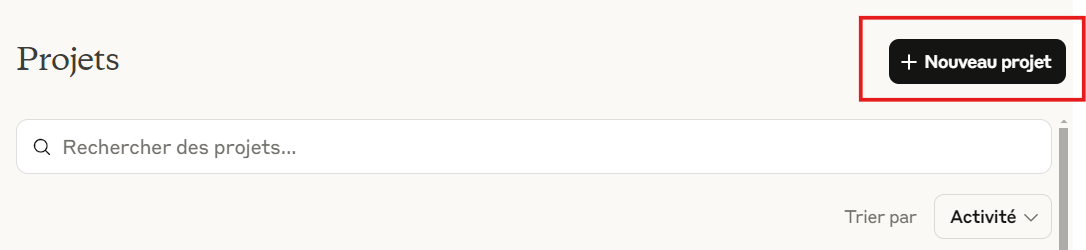
\includegraphics[width=0.75\textwidth]{images/Claude_setup_projects/new-project.png}\end{center}
        \tcbitem Décrire l'agent ( pour l'utilisateur seulement ). 

        \vspace{-0.3cm}\begin{center}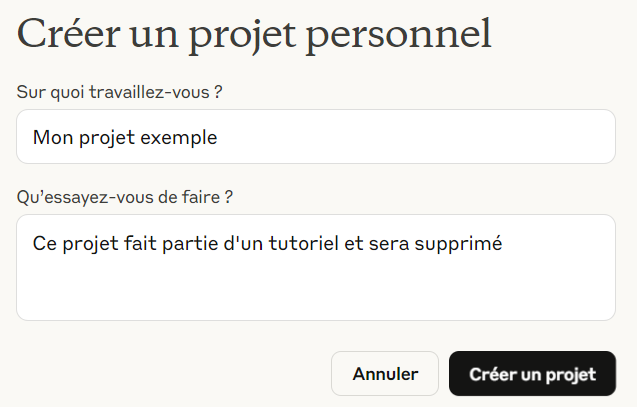
\includegraphics[width=0.55\textwidth]{images/Claude_setup_projects/base-setup.png}\end{center}
        \tcbitem Donner ses instructions. 

        \vspace{-0.3cm}\begin{center}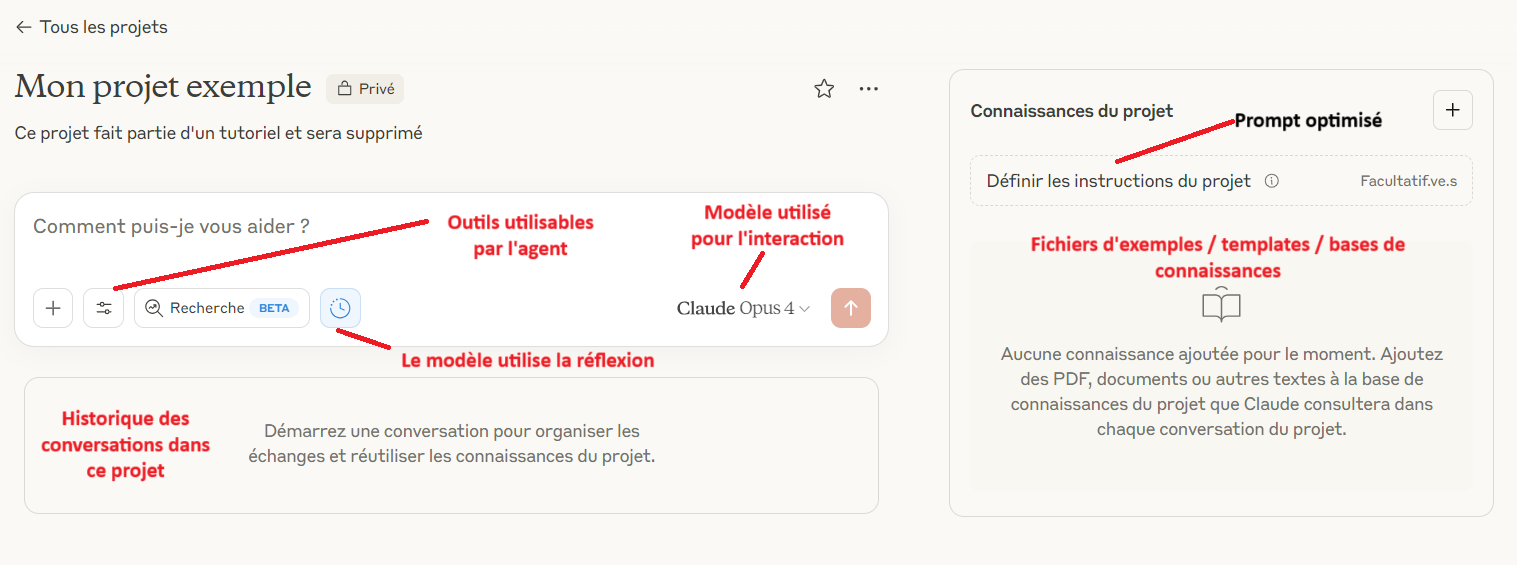
\includegraphics[width=0.95\textwidth]{images/Claude_setup_projects/complete-setup.png}\end{center}

        \tcbitem Votre agent est utilisable dans une \acc{nouvelle conversation}. 

        \vspace{-0.3cm}\begin{center}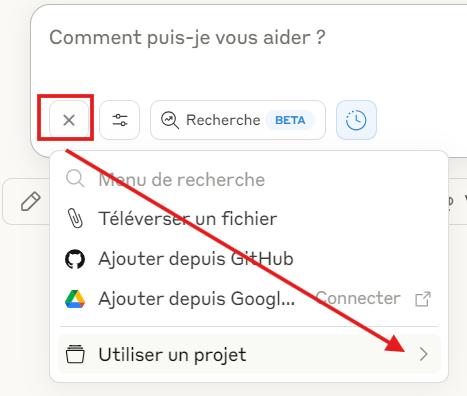
\includegraphics[width=0.55\textwidth]{images/Claude_setup_projects/use-setup.png}\end{center}
    \end{tcbenumerate}

    \begin{bfbox}{Mettre en place les MCP}
    \begin{tcbenumerate}[2]
        \tcbitem Accéder aux paramètres. 
        
        \vspace{-0.3cm}\begin{center}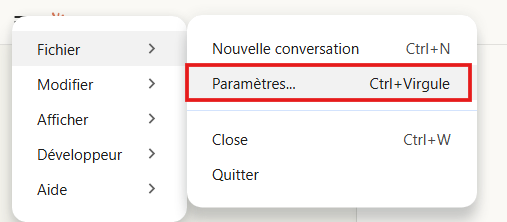
\includegraphics[width=0.55\textwidth]{images/Claude-setup-mcp/1.png}\end{center}
        \tcbitem Activer et accéder aux paramètres développeurs. 
        
        \vspace{-0.3cm}\begin{center}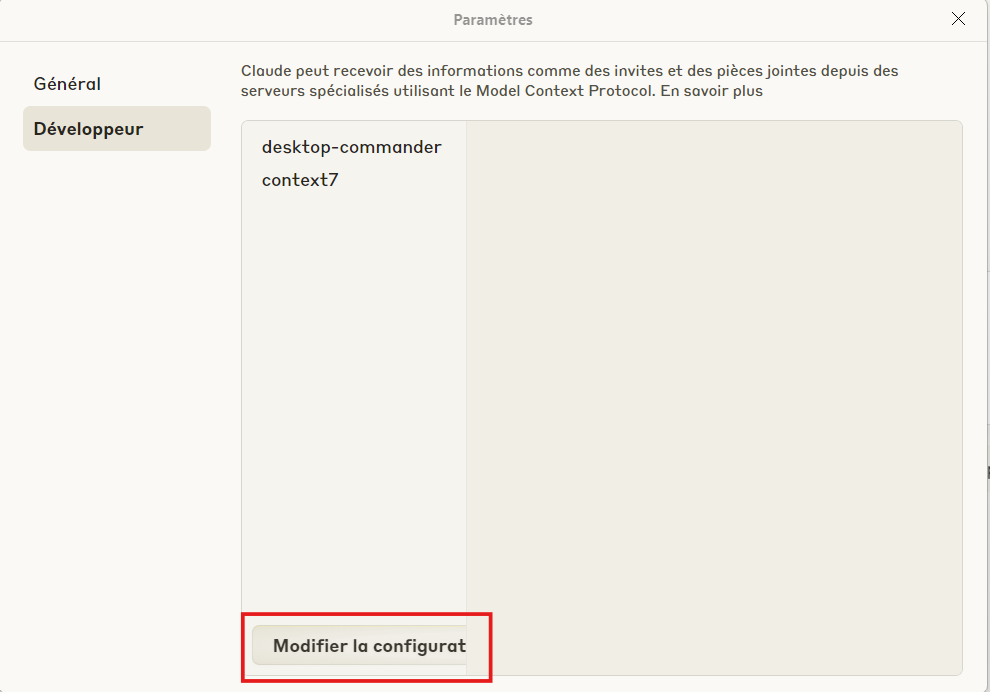
\includegraphics[width=0.55\textwidth]{images/Claude-setup-mcp/2.png}\end{center}
        \tcbitem Modifier le json des serveurs MCP comme donné dans les \acc{fichiers de la formation}.

        \vspace{-0.3cm}\begin{center}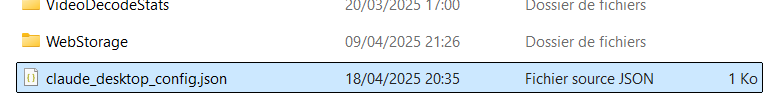
\includegraphics[width=0.55\textwidth]{images/Claude-setup-mcp/3.png}\end{center}

        \tcbitem Votre agent peut utiliser votre système de fichiers. 
    \end{tcbenumerate}
    \end{bfbox}
\end{Aide}

\begin{Aide}[Utiliser Windsurf ou Cursor]
    Ce sont des IDE comme VScode qui intègrent naturellement l'IA dans leur fonctionnement. Soutenus par de grandes entreprises une grande communauté de développeurs.

    On peut utiliser le même \acc{prompt system} que celui donné dans l'aide précédente. 
\end{Aide}

\begin{Aide}[Github Copilot]
    Ce modèle s'intègre bien dans VSCode et permet de la génération de code \LaTeX\ avec des suggestions. 

    Je ne l'utilise pas, mais c'est une solution plus discrète adaptée à ceux qui souhaitent rester maître du code écrit. 
    
    L'IA intervient pour \acc{suggérer} des modifications \acc{en contexte}. Il s'agit d'une alternative \acc{peu coûteuse}.
\end{Aide}


\subsection{Guidelines pour prompts structurés (2025)}

\begin{Definition}[Prompts structurés modernes]
    Les \voc{prompts structurés} représentent l'évolution des techniques de prompt engineering en 2025, combinant la précision du \acc{XML} pour la structure logique avec la lisibilité du \acc{Markdown} pour le contenu.
    
    Cette approche permet d'obtenir des réponses plus fiables et cohérentes des modèles de langage comme Claude d'Anthropic.
\end{Definition}

\begin{Methode}[Structure XML + Markdown]
    \begin{tcbraster}[raster columns=2,raster equal height=rows]
        \begin{tcolorbox}[title=Principe fondamental]
            \begin{itemize}[label=$\bullet$,itemsep=1.3em,leftmargin=*]
                \item \acc{XML} pour la \voc{structure logique}
                \item \acc{Markdown} pour le \voc{formatage du contenu}
                \item \voc{Balises sémantiques} descriptives
            \end{itemize}
        \end{tcolorbox}
        \begin{tcolorbox}[title=Exemple de base, colback=gray!5, colframe=gray!50]
            \ttfamily\small
            \xmltag{instructions}\\
            \hspace{1em}\#\# Tâche principale\\
            \hspace{1em}- Analyser le document\\
            \hspace{1em}- Extraire les points clés\\
            \hspace{1em}- **Formater** la sortie\\
            \xmlctag{instructions}
        \end{tcolorbox}
    \end{tcbraster}
\end{Methode}
\begin{Methode}[Ordre optimal des sections]
    L'ordre des sections dans un prompt structuré suit une progression logique du général au spécifique :
    
    \begin{tcbenumerate}[2]
        \tcbitem \xmltag{system_role} -- Qui est l'agent
        \tcbitem \xmltag{context} -- Situation et environnement  
        \tcbitem \xmltag{data} -- Données de référence
        \tcbitem \xmltag{rules} -- Règles et contraintes
        \tcbitem \xmltag{examples} -- Exemples few-shot
        \tcbitem \xmltag{instructions} -- Actions à effectuer
        \tcbitem \xmltag{output_format} -- Format de sortie
        \tcbitem \xmltag{critical_reminders} -- Points essentiels
    \end{tcbenumerate}
\end{Methode}

\begin{Exemple}[Prompt pour agent créateur de cartes \frquote{J'ai / Qui a}]
    Voici un exemple de prompt pour un agent spécialisé dans la création de cartes mathématiques :

    \begin{MultiColonnes}{2}
        \tcbitem \ttfamily\small
        \xmlbox{?xml version="1.0" encoding="UTF-8"?}\\[0.5em]
        \xmltag{agent_prompt}\\
        \hspace{1em}\xmltag{system_role}\\
        \hspace{2em}Expert LaTeX en création de jeux\\
        \hspace{2em}mathématiques pédagogiques\\
        \hspace{2em}Spécialiste tcolorbox et bfcours\\
        \hspace{1em}\xmlctag{system_role}\\[0.5em]
        \hspace{1em}\xmltag{context}\\
        \hspace{2em}\xmltag{level}Collège 4ème\xmlctag{level}\\
        \hspace{2em}\xmltag{topic}Calcul littéral\xmlctag{topic}\\
        \hspace{2em}\xmltag{cards_count}24\xmlctag{cards_count}\\
        \hspace{2em}\xmltag{objective}Jeu de révision\xmlctag{objective}\\
        \hspace{1em}\xmlctag{context}\\[0.5em]
        
        \tcbitem \ttfamily\small 
        \hspace{1em}\xmltag{instructions}\\
        \hspace{2em}\#\# Créer un jeu complet avec :\\
        \hspace{2em}1. **Cartes bouclées** (dernière $\rightarrow$ première)\\
        \hspace{2em}2. **Progression** de difficulté\\
        \hspace{2em}3. **Variété** des expressions\\[0.5em]
        \hspace{2em}\#\# Contraintes techniques :\\
        \hspace{2em}- Utiliser \textbackslash{}definecolor\{cardcolor\}\\
        \hspace{2em}- Format A4 avec 8 cartes/page\\
        \hspace{2em}- Police lisible (12pt minimum)\\
        \hspace{1em}\xmlctag{instructions}\\[0.5em]
        \hspace{1em}\xmltag{card_structure}\\
        \hspace{2em}\xmltag{front}J'ai : [expression]\xmlctag{front}\\
        \hspace{2em}\xmltag{back}Qui a : [question]\xmlctag{back}\\
        \hspace{1em}\xmlctag{card_structure}
    \end{MultiColonnes}
\end{Exemple}
\vspace{-0.5cm}\begin{Remarque}[Anti-patterns à éviter]
    \vspace{-0.5cm}\begin{Colonnes}[2]%[raster columns=2, raster equal height]
        \begin{tcolorbox}[title={\textcolor{red!75!white}{\textcolor{red}{\faTimes} À éviter}}, colback=red!5]
            \begin{itemize}[label=$\times$]
                \item Instructions négatives excessives (\frquote{Ne fais pas...})
                \item Balises XML invalides ou mal fermées
                \item Mélange contexte/instructions
                \item Exemples incohérents en format
                \item Instructions incohérentes
            \end{itemize}
        \end{tcolorbox}
        \begin{tcolorbox}[title={\textcolor{green!70!black}{$\checkmark$ Bonnes pratiques}}, colback=green!5]
            \begin{itemize}[label=$\checkmark$]
                \item Instructions positives claires
                \item Structure XML valide et cohérente
                \item Séparation nette des sections
                \item Exemples uniformes
                \item Concision, précision et cohérence
            \end{itemize}
        \end{tcolorbox}
    \end{Colonnes}
\end{Remarque}
\begin{Methode}[Techniques avancées]
    \begin{MultiColonnes}{2}
        \tcbitem \textbf{Chain of Thought} 

        Technique permettant de décomposer le raisonnement :
        
        \begin{tcolorbox}[colback=gray!5, colframe=gray!50]
            \ttfamily\small
            \xmltag{thinking_process}\\
            \hspace{1em}1. D'abord, analyser...\\
            \hspace{1em}2. Ensuite, vérifier...\\
            \hspace{1em}3. Finalement, produire...\\
            \xmlctag{thinking_process}
        \end{tcolorbox}
        \tcbitem \textbf{Scratchpad} 

        Pour les documents longs, utiliser un bloc-notes :

        \vfill
        \begin{tcolorbox}[colback=gray!5, colframe=gray!50]
            \ttfamily\small
            \xmltag{scratchpad}\\
            \hspace{1em}Points clés à retenir :\\
            \hspace{1em}- Information critique 1\\
            \hspace{1em}- Donnée importante 2\\
            \xmlctag{scratchpad}
        \end{tcolorbox}
    \end{MultiColonnes}
    \begin{tcolorbox}[title=Scratchpad permanent :,colback=gray!5, colframe=gray!50]
        \ttfamily\small
        \xmltag{scratchpad}\\
        \hspace{1em}Utilise le fichier \displayFilePath{mon\_repertoire\_IA/AI\_NOTES.xml} pour :\\
        \hspace{1em}- Noter ton plan d'action\\
        \hspace{1em}- Tenir à jour les étapes effectuées au fur et à mesure.\\
        \xmlctag{scratchpad}
    \end{tcolorbox}
    \encadrer[purple]{Cette dernière méthode est extrêmement efficace et permet aux agents de se succéder de façon fluide.}
\end{Methode}

\begin{Methode}[Prompt optimisé]
    Adapter la structure selon le type de tâche :
    
    \begin{MultiColonnes}{3}[colframe=\itemBaseColor,boxrule=0.4pt]
        \tcbitem[title=Pour du code,halign=left] 
        \begin{itemize}[label=$\bullet$,leftmargin=*]
            \item Structure de fichiers attendue
            \item Conventions de nommage
            \item Exemples d'entrée/sortie
        \end{itemize}
        \tcbitem[title=Pour des documents] 
        \begin{itemize}[label=$\bullet$]
            \item Templates de structure
            \item Styles d'écriture
            \item Ton et registre
        \end{itemize}
        \tcbitem[title=Pour des analyses] 
        \begin{itemize}[label=$\bullet$]
            \item Critères d'évaluation
            \item Métriques à calculer
            \item Format de rapport
        \end{itemize}
    \end{MultiColonnes}

    Pour un agent spécialisé en \LaTeX\ avec \acc{bfcours}, voici la structure optimale :
        \dirtree{%
            .1 \xmltag{latex_agent_prompt}.
            .2 \xmltag{system_role} \DTcomment{\color{green!75!black}Expert LaTeX/bfcours}.
            .2 \xmltag{context} \DTcomment{\color{green!75!black}Environnement pédagogique}.
            .2 \xmltag{bfcours_conventions}.
            .3 \xmltag{environments} \DTcomment{\color{green!75!black}Definition, Exemple, etc.}.
            .3 \xmltag{commands} \DTcomment{\color{green!75!black}\textbackslash voc, \textbackslash acc, etc.}.
            .3 \xmltag{layout} \DTcomment{\color{green!75!black}MultiColonnes, tcbraster}.
            .2 \xmltag{quality_requirements}.
            .3 \xmltag{imperative_rules} \DTcomment{\color{green!75!black}Règles strictes}.
            .3 \xmltag{design_principles} \DTcomment{\color{green!75!black}Principes de design}.
            .2 \xmltag{workflow_instructions}.\DTcomment{\color{green!75!black}Patterns de travail / chaîne de pensée}.
            .2 \xmltag{critical_reminders}.\DTcomment{\color{green!75!black}Points clés à respecter ( synthétique )}.
        }
\end{Methode}
\begin{bfbox}{Processus d'itération}
    \begin{tcbenumerate}[2]
        \tcbitem \textbf{Tester} avec des cas limites variés
        \tcbitem \textbf{Analyser} les échecs et réussites
        \tcbitem \textbf{Enrichir progressivement} la structure et les instructions
        \tcbitem \textbf{Affiner} le prompt
        \tcbitem \textbf{Conserver} une bibliothèque de prompts testés
        \tcbitem \textbf{Partager} les agents efficaces découverts
    \end{tcbenumerate}
    %\vspace{-0.6cm}
    \begin{center}
        \acc{Règle d'or :}
    \encadrer[\itemBaseColor]{Un prompt bien structuré}
            {\huge =}
            \encadrer[\itemBaseColor]{Moins de corrections} 
            {\huge +} 
            \encadrer[\itemBaseColor]{Meilleure productivité}\\

        \encadrer[cyan]{\frquote{La structure parfaite émerge de l'expérimentation continue.}}
    \end{center}

    
\end{bfbox}
\newpage
\subsection{Adapter bfcours à ses besoins}

\begin{Methode}[Créer votre propre package]
 \begin{MultiColonnes}{3}
    \tcbitem[raster multicolumn=2] Il convient de créer votre propre package pour apporter vos modifications de façon globale. 

Il suffira alors de l'utiliser dans vos documents : 

\showcmd{usepackage}[\{bfcours\}]

\showcmd{usepackage}[\{adapt-bfcours\}]\mycomment{Votre package qui modifiera bfcours}

    \tcbitem \bclampe On pourra consulter l'archive suivante : \vocnoindexref{https://tuteurs.ens.fr/logiciels/latex/nouveau_package.html}{archives tuteurs ENS}.
 \end{MultiColonnes}
\end{Methode}
\begin{Methode}[Personnaliser un package]
Puisque \LaTeX\ est orienté vers la personnalisation, il est possible d'adapter n'importe quel package à vos besoins. 
Il y a plusieurs façons de procéder : 
\begin{tcbenumerate}[2]
    \tcbitem Créer vos propres commandes qui simplifient l'utilisation de celles données dans les packages utilisés. 

    \mycomment{définition d'origine}

    \showcmd{newcommand}[\{$\backslash$bonjour\}[1]\{Bonjour, \#1\}] 

    \mycomment{définition que vous utiliserez}

    \showcmd{newcommand}[\{$\backslash$mybonjour\}[1]\{$\backslash$bonjour\{\#1\} !\}] 

    \tcbitem Réécrire certaines commandes pour qu'elles agissent différemment. 

    Cela peut être une tâche ardue, parfois il faut retrouver le code d'origine de la commande, recopier son contenu et modifier la copie. 

    \mycomment{définition d'origine}

    \showcmd{newcommand}[\{$\backslash$bonjour\}\{bonjour\}] 

    \mycomment{On réécrit la définition de la commande}

    \showcmd{renewcommand}[\{$\backslash$bonjour\}\{Bonjour !\}] 
\end{tcbenumerate}
\end{Methode}

\begin{Methode}[Naviguer dans un package]
    Il est très \acc{utile} et \acc{formateur} de lire directement le code source des packages qu'on utilise. 

    \bfcours\ propose un \acc{programme de recherche} de définition de commande \LaTeX\ dans un package donné ( configurable par l'utilisateur ).

    Il permet de \acc{saisir le nom d'une commande}, d'\acc{environnement} ou de \acc{couleur} et s'il trouve sa définition, il \acc{ouvre} VSCode à la ligne trouvée.

    Il suffit de lire le fichier suivant et d'utiliser les commandes données.
    
    \displayFilePath{fichiers\_de\_la\_formation/programmes/Commandes\_de\_recherche\_dans\_un\_package/README.md}

    \encadrer[green]{Ce programme de recherche de code à été entièrement écrit par Claude.}
\end{Methode}
\subsection{Logiciel comme générateur de code LaTeX}

\begin{tcolorbox}[blank]
    
    L'utilisation de logiciels qui génèrent du code \LaTeX\ est une idée permettant de reléguer le côté fastidieux au second plan. 

Le mode d'action est relativement simple : 
\begin{tcbenumerate}
    \tcbitem Choisir un langage que vous maîtrisez un peu ( Python, javascript... )
    \tcbitem Lister les morceaux de code \LaTeX\ à produire. Plus vous avez d'exemples, mieux c'est. 
    \tcbitem Produire éventuellement un modèle \LaTeX\ que le logiciel viendra \acc{modifier}.
    \tcbitem Demander à l'IA de produire un script permettant de générer un document \LaTeX\ sur base de vos instructions.
    \tcbitem Testez, débuguez, modifiez et demander à l'IA d'améliorer son code grâce à vos retours.
\end{tcbenumerate}

On peut trouver beaucoup de cas d'utilisation : 

\begin{MultiColonnes}{4}[colframe=black,boxrule=0.4pt,colback=gray!5!white]%


    \tcbitem[colback=blue!10!white] Production de cartes
    \tcbitem[colback=green!10!white] Gestion des modèles
    \tcbitem[colback=yellow!10!white] Gestion d'une banque de questions
    \tcbitem[colback=yellow!10!white] Abstraction d'exercices pour produire plusieurs versions
    \tcbitem[colback=yellow!10!white] Produire des ressources générées procéduralement ( puzzles, carrés magiques... )
    \tcbitem[colback=yellow!10!white] Analyser du code \LaTeX\ et le modifier ( mise à jour de fichiers anciens ). 
    \tcbitem[colback=green!10!white] Retrouver la définition d'une commande spécifique. 
    \tcbitem[colback=green!10!white] Produire des rapports d'analyse d'évaluation.
\end{MultiColonnes}

Code couleur :

\begin{MultiColonnes}{3}% 
    \tcbitem[colback=yellow!10!white] En cours de production par \bfcours.
    \tcbitem[colback=blue!10!white] Solution disponible dans \bfcours\ mais à personnaliser.
    \tcbitem[colback=green!10!white] Solution disponible dans \bfcours.
\end{MultiColonnes}
\end{tcolorbox}

\newpage
\section{Annexes}

\subsection{Exemple d'utilisation de Claude}

\begin{bfbox}{La création des \frquote{\textsc{toolbox}}}

    Pour fournir les kits d'outils des exercices de cette formation, j'ai demandé à Claude code de me préparer des designs dont je pourrais m'inspirer. 

    J'ai utilisé l'agent scripteur décrit dans cette formation. 

    \begin{tcbenumerate}[2]
        \tcbitem \acc{Le prompt}. \mycomment{On ne s'est pas appliqué. C'est possible grâce à la qualité du pré-prompt.}
        \begin{center}
        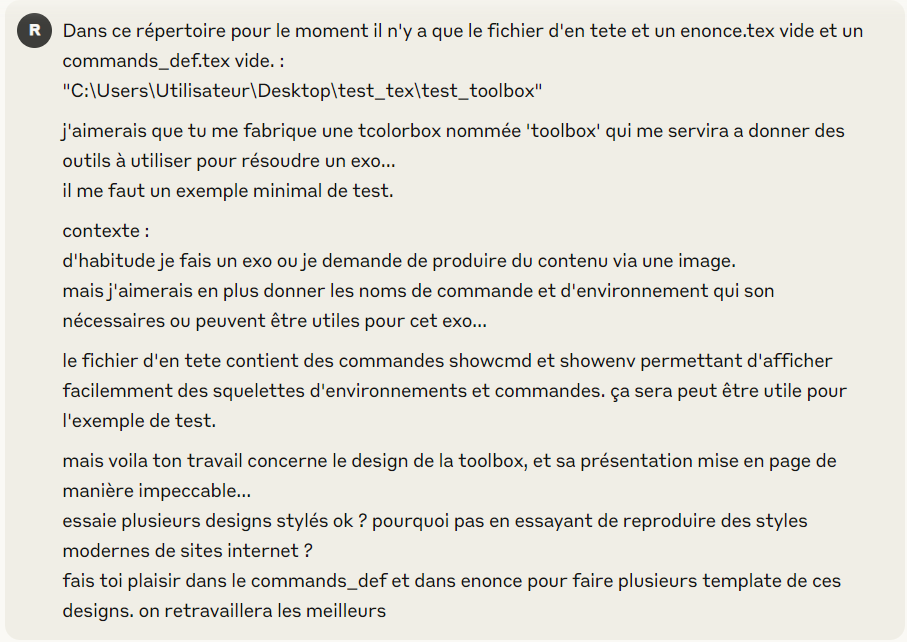
\includegraphics[width=0.75\textwidth]{annexes/Example_craft_toolbox/1.png}
        \end{center}
        
        \tcbitem \acc{L'action'}. \mycomment{Le modèle analyse le contenu, puis agis. Il tente même de compiler avec plusieurs compilateurs.}
        \begin{center}
        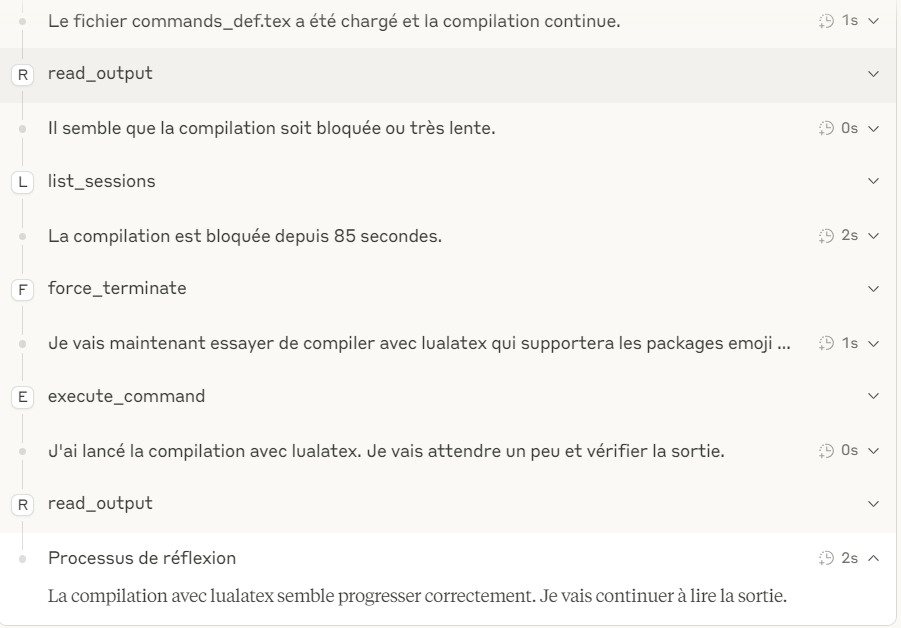
\includegraphics[width=0.75\textwidth]{annexes/Example_craft_toolbox/3.png}
        \end{center}

        \tcbitem \acc{Le rendu}. \mycomment{Claude a été efficace, je n'ai plus qu'à choisir parmi les $8$ exemples fournis.}
        \begin{center}
        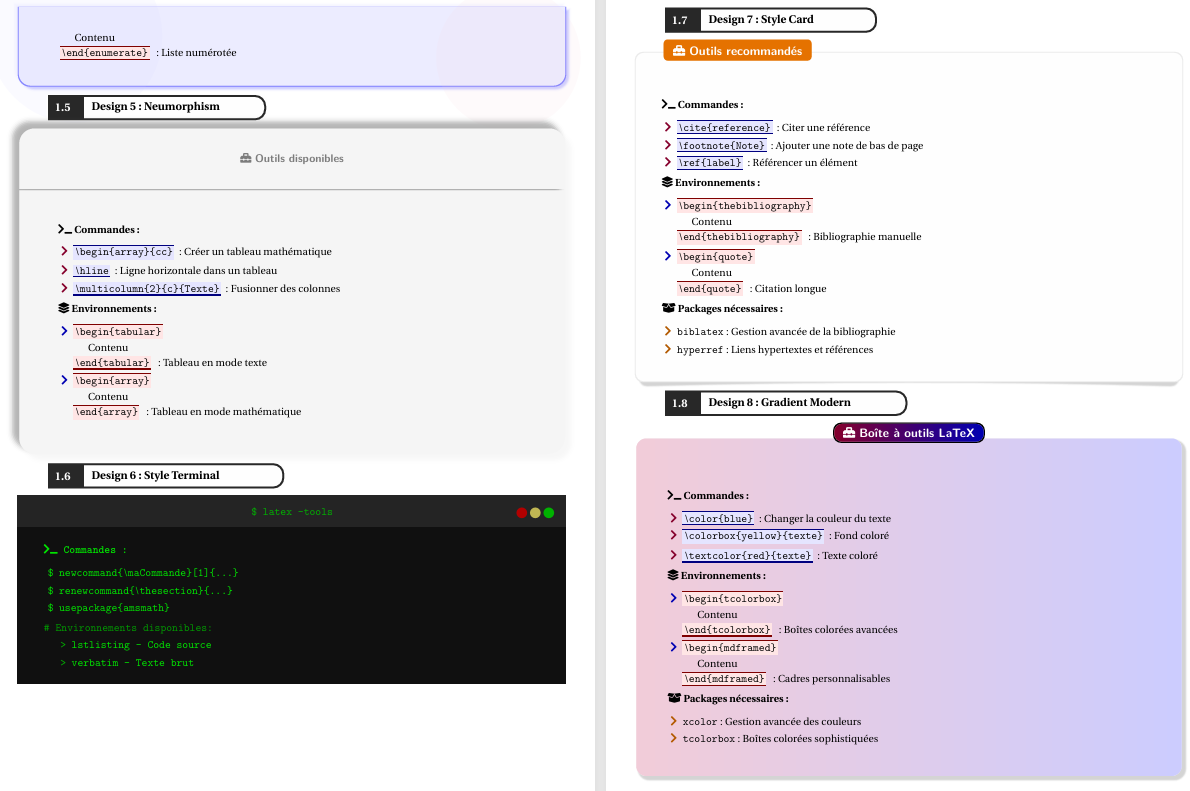
\includegraphics[width=0.75\textwidth]{annexes/Example_craft_toolbox/4.png}
        \end{center}     
        
        \tcbitem \acc{L'investissement en temps} :

        En regardant les propriétés du dossier de test pour ces exemples de design, on a :  
        \begin{itemize}[label=$\bullet$]
            \item \encadrer{Date de création : 8h23}
        
            \item \encadrer[green]{Date de fin d'édition de cet exemple : 9h}
        \end{itemize}

        La création de cet exemple et du design des mes \textsc{toolbox} n'a pris qu'un peu plus d'une demi-heure.
    \end{tcbenumerate}
\end{bfbox}